% Options for packages loaded elsewhere
\PassOptionsToPackage{unicode}{hyperref}
\PassOptionsToPackage{hyphens}{url}
%
\documentclass[
]{article}
\usepackage{amsmath,amssymb}
\usepackage{lmodern}
\usepackage{iftex}
\ifPDFTeX
  \usepackage[T1]{fontenc}
  \usepackage[utf8]{inputenc}
  \usepackage{textcomp} % provide euro and other symbols
\else % if luatex or xetex
  \usepackage{unicode-math}
  \defaultfontfeatures{Scale=MatchLowercase}
  \defaultfontfeatures[\rmfamily]{Ligatures=TeX,Scale=1}
\fi
% Use upquote if available, for straight quotes in verbatim environments
\IfFileExists{upquote.sty}{\usepackage{upquote}}{}
\IfFileExists{microtype.sty}{% use microtype if available
  \usepackage[]{microtype}
  \UseMicrotypeSet[protrusion]{basicmath} % disable protrusion for tt fonts
}{}
\makeatletter
\@ifundefined{KOMAClassName}{% if non-KOMA class
  \IfFileExists{parskip.sty}{%
    \usepackage{parskip}
  }{% else
    \setlength{\parindent}{0pt}
    \setlength{\parskip}{6pt plus 2pt minus 1pt}}
}{% if KOMA class
  \KOMAoptions{parskip=half}}
\makeatother
\usepackage{xcolor}
\usepackage[margin=1in]{geometry}
\usepackage{color}
\usepackage{fancyvrb}
\newcommand{\VerbBar}{|}
\newcommand{\VERB}{\Verb[commandchars=\\\{\}]}
\DefineVerbatimEnvironment{Highlighting}{Verbatim}{commandchars=\\\{\}}
% Add ',fontsize=\small' for more characters per line
\usepackage{framed}
\definecolor{shadecolor}{RGB}{248,248,248}
\newenvironment{Shaded}{\begin{snugshade}}{\end{snugshade}}
\newcommand{\AlertTok}[1]{\textcolor[rgb]{0.94,0.16,0.16}{#1}}
\newcommand{\AnnotationTok}[1]{\textcolor[rgb]{0.56,0.35,0.01}{\textbf{\textit{#1}}}}
\newcommand{\AttributeTok}[1]{\textcolor[rgb]{0.77,0.63,0.00}{#1}}
\newcommand{\BaseNTok}[1]{\textcolor[rgb]{0.00,0.00,0.81}{#1}}
\newcommand{\BuiltInTok}[1]{#1}
\newcommand{\CharTok}[1]{\textcolor[rgb]{0.31,0.60,0.02}{#1}}
\newcommand{\CommentTok}[1]{\textcolor[rgb]{0.56,0.35,0.01}{\textit{#1}}}
\newcommand{\CommentVarTok}[1]{\textcolor[rgb]{0.56,0.35,0.01}{\textbf{\textit{#1}}}}
\newcommand{\ConstantTok}[1]{\textcolor[rgb]{0.00,0.00,0.00}{#1}}
\newcommand{\ControlFlowTok}[1]{\textcolor[rgb]{0.13,0.29,0.53}{\textbf{#1}}}
\newcommand{\DataTypeTok}[1]{\textcolor[rgb]{0.13,0.29,0.53}{#1}}
\newcommand{\DecValTok}[1]{\textcolor[rgb]{0.00,0.00,0.81}{#1}}
\newcommand{\DocumentationTok}[1]{\textcolor[rgb]{0.56,0.35,0.01}{\textbf{\textit{#1}}}}
\newcommand{\ErrorTok}[1]{\textcolor[rgb]{0.64,0.00,0.00}{\textbf{#1}}}
\newcommand{\ExtensionTok}[1]{#1}
\newcommand{\FloatTok}[1]{\textcolor[rgb]{0.00,0.00,0.81}{#1}}
\newcommand{\FunctionTok}[1]{\textcolor[rgb]{0.00,0.00,0.00}{#1}}
\newcommand{\ImportTok}[1]{#1}
\newcommand{\InformationTok}[1]{\textcolor[rgb]{0.56,0.35,0.01}{\textbf{\textit{#1}}}}
\newcommand{\KeywordTok}[1]{\textcolor[rgb]{0.13,0.29,0.53}{\textbf{#1}}}
\newcommand{\NormalTok}[1]{#1}
\newcommand{\OperatorTok}[1]{\textcolor[rgb]{0.81,0.36,0.00}{\textbf{#1}}}
\newcommand{\OtherTok}[1]{\textcolor[rgb]{0.56,0.35,0.01}{#1}}
\newcommand{\PreprocessorTok}[1]{\textcolor[rgb]{0.56,0.35,0.01}{\textit{#1}}}
\newcommand{\RegionMarkerTok}[1]{#1}
\newcommand{\SpecialCharTok}[1]{\textcolor[rgb]{0.00,0.00,0.00}{#1}}
\newcommand{\SpecialStringTok}[1]{\textcolor[rgb]{0.31,0.60,0.02}{#1}}
\newcommand{\StringTok}[1]{\textcolor[rgb]{0.31,0.60,0.02}{#1}}
\newcommand{\VariableTok}[1]{\textcolor[rgb]{0.00,0.00,0.00}{#1}}
\newcommand{\VerbatimStringTok}[1]{\textcolor[rgb]{0.31,0.60,0.02}{#1}}
\newcommand{\WarningTok}[1]{\textcolor[rgb]{0.56,0.35,0.01}{\textbf{\textit{#1}}}}
\usepackage{longtable,booktabs,array}
\usepackage{calc} % for calculating minipage widths
% Correct order of tables after \paragraph or \subparagraph
\usepackage{etoolbox}
\makeatletter
\patchcmd\longtable{\par}{\if@noskipsec\mbox{}\fi\par}{}{}
\makeatother
% Allow footnotes in longtable head/foot
\IfFileExists{footnotehyper.sty}{\usepackage{footnotehyper}}{\usepackage{footnote}}
\makesavenoteenv{longtable}
\usepackage{graphicx}
\makeatletter
\def\maxwidth{\ifdim\Gin@nat@width>\linewidth\linewidth\else\Gin@nat@width\fi}
\def\maxheight{\ifdim\Gin@nat@height>\textheight\textheight\else\Gin@nat@height\fi}
\makeatother
% Scale images if necessary, so that they will not overflow the page
% margins by default, and it is still possible to overwrite the defaults
% using explicit options in \includegraphics[width, height, ...]{}
\setkeys{Gin}{width=\maxwidth,height=\maxheight,keepaspectratio}
% Set default figure placement to htbp
\makeatletter
\def\fps@figure{htbp}
\makeatother
\usepackage[normalem]{ulem}
\setlength{\emergencystretch}{3em} % prevent overfull lines
\providecommand{\tightlist}{%
  \setlength{\itemsep}{0pt}\setlength{\parskip}{0pt}}
\setcounter{secnumdepth}{-\maxdimen} % remove section numbering
\usepackage{booktabs}
\usepackage{longtable}
\usepackage{array}
\usepackage{multirow}
\usepackage{wrapfig}
\usepackage{float}
\usepackage{colortbl}
\usepackage{pdflscape}
\usepackage{tabu}
\usepackage{threeparttable}
\usepackage{threeparttablex}
\usepackage[normalem]{ulem}
\usepackage{makecell}
\usepackage{xcolor}
\ifLuaTeX
  \usepackage{selnolig}  % disable illegal ligatures
\fi
\IfFileExists{bookmark.sty}{\usepackage{bookmark}}{\usepackage{hyperref}}
\IfFileExists{xurl.sty}{\usepackage{xurl}}{} % add URL line breaks if available
\urlstyle{same} % disable monospaced font for URLs
\hypersetup{
  pdftitle={Analyse des données de consommations d'énergie en Inde},
  hidelinks,
  pdfcreator={LaTeX via pandoc}}

\title{Analyse des données de consommations d'énergie en Inde}
\author{}
\date{\vspace{-2.5em}}

\begin{document}
\maketitle

\hypertarget{environnement-de-travail}{%
\section{Environnement de travail}\label{environnement-de-travail}}

\begin{Shaded}
\begin{Highlighting}[]
\FunctionTok{library}\NormalTok{(tidyverse)}
\FunctionTok{library}\NormalTok{(ggplot2)}
\FunctionTok{library}\NormalTok{(readxl)}
\FunctionTok{library}\NormalTok{(tidyr)}
\FunctionTok{library}\NormalTok{(fda)}
\FunctionTok{library}\NormalTok{(knitr)}
\FunctionTok{library}\NormalTok{(kableExtra)}
\end{Highlighting}
\end{Shaded}

\hypertarget{i.-notre-base-de-donnuxe9es}{%
\section{I. Notre base de données}\label{i.-notre-base-de-donnuxe9es}}

Notre étude porte sur l'analyse de la consommation d'énergie dans les 33
Etats d'Inde. Il est à noter que l'Inde est le troisième producteur et
le troisième consommateur d'électricité au monde.\\
Nous avons choisi ce sujet car il est au coeur des problématiques
sociétales actuelles. En effet, dans les politiques actuelles, la
question de l'environnement a une part importante. Notamment, la gestion
de l'énergie pour les pays avec une forte croissance de population comme
l'Inde. Notre étude peut mettre en avant les comportements de
consommation des différents Etats et inciter à réfléchir sur la
problématique de l'optimisation de cette consommation.

Ce projet nous permet d'appliquer nos connaissances à des thématiques
concrètes dans le monde professionnel.

\hypertarget{i.a.-importation-des-donnuxe9es}{%
\subsection{I.A. Importation des
données}\label{i.a.-importation-des-donnuxe9es}}

Dans un premier temps, nous allons importer les données.

\begin{Shaded}
\begin{Highlighting}[]
\NormalTok{data }\OtherTok{\textless{}{-}} \FunctionTok{read.csv}\NormalTok{(}\StringTok{"long\_data\_2.csv"}\NormalTok{, }\AttributeTok{stringsAsFactors =}\NormalTok{ T,}\AttributeTok{sep =} \StringTok{";"}\NormalTok{)}

\FunctionTok{colnames}\NormalTok{(data) }\OtherTok{\textless{}{-}} \FunctionTok{c}\NormalTok{(}\StringTok{"Etat"}\NormalTok{, }\StringTok{"Regions"}\NormalTok{, }\StringTok{"latitude"}\NormalTok{, }\StringTok{"longitude"}\NormalTok{, }
                    \StringTok{"Date"}\NormalTok{, }\StringTok{"Consommation"}\NormalTok{) }\CommentTok{\# renommage des colonnes}

\NormalTok{data }\OtherTok{\textless{}{-}}\NormalTok{ data[,}\SpecialCharTok{{-}}\FunctionTok{c}\NormalTok{(}\DecValTok{3}\NormalTok{,}\DecValTok{4}\NormalTok{)]}
\FunctionTok{summary}\NormalTok{(data)}
\end{Highlighting}
\end{Shaded}

\begin{verbatim}
##                 Etat       Regions                  Date        Consommation  
##  Andhra Pradesh   :  498   ER :2490   01/01/2020 00:00:   33   Min.   :  0.3  
##  Arunachal Pradesh:  498   NER:3486   01/02/2020 00:00:   33   1st Qu.:  6.7  
##  Assam            :  498   NR :4482   01/03/2020 00:00:   33   Median : 64.5  
##  Bihar            :  498   SR :2988   01/04/2020 00:00:   33   Mean   :103.1  
##  Chandigarh       :  498   WR :2988   01/05/2020 00:00:   33   3rd Qu.:174.0  
##  Chhattisgarh     :  498              01/06/2020 00:00:   33   Max.   :522.1  
##  (Other)          :13446              (Other)         :16236
\end{verbatim}

\begin{Shaded}
\begin{Highlighting}[]
\CommentTok{\# View(data)}
\end{Highlighting}
\end{Shaded}

\begin{Shaded}
\begin{Highlighting}[]
\FunctionTok{dim}\NormalTok{(data)}
\end{Highlighting}
\end{Shaded}

\begin{verbatim}
## [1] 16434     4
\end{verbatim}

Concernant notre base de données, elle décrit la consommation d'énergie
dans \textbf{33 Etats} d'Inde entre 2019 et 2020.\\
Nous avons 16 434 lignes, soit \textbf{498 points de mesure} par pays
(498*33). Les données sont journalières, exprimées en Mega Units.

Grâce au résumé statistique ci-dessus, nous pouvons voir que les valeurs
de nos données de consommation d'énergie sont assez étendues : elles
sont comprises entre 0.3 et 522.1 Mega Units. La consommation moyenne en
Inde est de 103.1 Mega Units en comparaison avec la médiane qui est de
64.5 Mega Units. Ainsi, la moyenne est très influencée par les valeurs
extrêmes de certains Etats de notre jeu de données.\\

\begin{Shaded}
\begin{Highlighting}[]
\NormalTok{data}\SpecialCharTok{$}\NormalTok{Etat[}\FunctionTok{which.max}\NormalTok{(data}\SpecialCharTok{$}\NormalTok{Consommation)]}
\end{Highlighting}
\end{Shaded}

\begin{verbatim}
## [1] Maharashtra
## 33 Levels: Andhra Pradesh Arunachal Pradesh Assam Bihar ... West Bengal
\end{verbatim}

\begin{Shaded}
\begin{Highlighting}[]
\NormalTok{data}\SpecialCharTok{$}\NormalTok{Etat[}\FunctionTok{which.min}\NormalTok{(data}\SpecialCharTok{$}\NormalTok{Consommation)]}
\end{Highlighting}
\end{Shaded}

\begin{verbatim}
## [1] Sikkim
## 33 Levels: Andhra Pradesh Arunachal Pradesh Assam Bihar ... West Bengal
\end{verbatim}

En effet, certaines valeurs journalières sont très faibles (inférieures
à 1) alors que d'autres sont 500 fois plus élevées. Par exemple, le
Maharashtra qui présente certaines valeurs très importantes en
opposition avec le Sikkim.

\hypertarget{i.b.-choix-de-la-puxe9riode-uxe9tudiuxe9e}{%
\subsection{I.B. Choix de la période
étudiée}\label{i.b.-choix-de-la-puxe9riode-uxe9tudiuxe9e}}

Nous allons transformer notre variable Date au format date pour
poursuivre l'étude correctement.

\begin{Shaded}
\begin{Highlighting}[]
\NormalTok{data}\SpecialCharTok{$}\NormalTok{Date }\OtherTok{\textless{}{-}} \FunctionTok{as.Date}\NormalTok{(data}\SpecialCharTok{$}\NormalTok{Date, }\AttributeTok{format =} \StringTok{"\%d/\%m/\%Y \%H:\%M"}\NormalTok{)}
\FunctionTok{str}\NormalTok{(data) }\CommentTok{\# Vérification}
\end{Highlighting}
\end{Shaded}

\begin{verbatim}
## 'data.frame':    16434 obs. of  4 variables:
##  $ Etat        : Factor w/ 33 levels "Andhra Pradesh",..: 25 11 26 7 31 32 12 13 5 6 ...
##  $ Regions     : Factor w/ 5 levels "ER","NER","NR",..: 3 3 3 3 3 3 3 3 3 5 ...
##  $ Date        : Date, format: "2019-01-02" "2019-01-02" ...
##  $ Consommation: num  119.9 130.3 234.1 85.8 313.9 ...
\end{verbatim}

Pour simplifier notre analyse, nous allons nous concentrer seulement sur
l'année 2019 :

\begin{Shaded}
\begin{Highlighting}[]
\NormalTok{data }\OtherTok{\textless{}{-}}\NormalTok{ data }\SpecialCharTok{|\textgreater{}} 
  \FunctionTok{filter}\NormalTok{(Date }\SpecialCharTok{\textless{}=} \FunctionTok{as.Date}\NormalTok{(}\StringTok{"2020{-}01{-}02"}\NormalTok{))}
\end{Highlighting}
\end{Shaded}

On vérifie à présent que les données que l'on va analyser correspondent
bien à la période choisie.

\begin{Shaded}
\begin{Highlighting}[]
\FunctionTok{min}\NormalTok{(data}\SpecialCharTok{$}\NormalTok{Date)}
\end{Highlighting}
\end{Shaded}

\begin{verbatim}
## [1] "2019-01-02"
\end{verbatim}

\begin{Shaded}
\begin{Highlighting}[]
\FunctionTok{max}\NormalTok{(data}\SpecialCharTok{$}\NormalTok{Date)}
\end{Highlighting}
\end{Shaded}

\begin{verbatim}
## [1] "2020-01-02"
\end{verbatim}

Notre étude porte sur la période du 02 Janvier 2019 au 02 Janvier
2020.\\
Nous avons pu observer que les données du 1er de chaque mois sont
manquantes mais cela n'impactera pas notre analyse.

\hypertarget{i.c.-normalisation-des-donnuxe9es}{%
\subsection{I.C. Normalisation des
données}\label{i.c.-normalisation-des-donnuxe9es}}

Au départ, nous avons voulu normaliser les données par le nombre
d'habitants de chaque Etat pour que les consommations aient le même
impact dans notre étude. Cependant, cette méthode s'est révélée
problématique car nous avons obtenu des valeurs très proches de zéro, ce
qui aurait compliqué les calculs.

Nous avons donc choisi de réduire les données de consommation, en
soustrayant la moyenne, pour continuer notre analyse avec données moins
disproportionnées.

\begin{Shaded}
\begin{Highlighting}[]
\NormalTok{moyenne\_par\_etat }\OtherTok{\textless{}{-}} \FunctionTok{tapply}\NormalTok{(data}\SpecialCharTok{$}\NormalTok{Consommation, data}\SpecialCharTok{$}\NormalTok{Etat, mean)}

\NormalTok{normalized\_energy }\OtherTok{\textless{}{-}}\NormalTok{ data}
\ControlFlowTok{for}\NormalTok{(i }\ControlFlowTok{in} \DecValTok{1}\SpecialCharTok{:}\FunctionTok{nrow}\NormalTok{(normalized\_energy))\{}
\NormalTok{  normalized\_energy}\SpecialCharTok{$}\NormalTok{Consommation[i] }\OtherTok{\textless{}{-}}\NormalTok{ normalized\_energy}\SpecialCharTok{$}\NormalTok{Consommation[i] }\SpecialCharTok{{-}}\NormalTok{ moyenne\_par\_etat[normalized\_energy}\SpecialCharTok{$}\NormalTok{Etat[i]]}
\NormalTok{\}}
\FunctionTok{head}\NormalTok{(normalized\_energy)}
\end{Highlighting}
\end{Shaded}

Suite à cette normailisation, nous pouvons observer une diminution
importante des valeurs. Mais nous obtenons des valeurs de consommations
négatives, ce qui pose problème pour l'interprétation de nos analyses.
De plus, mettre les données en valeur absolue n'aurait pas de sens dans
notre contxte. Nous avons donc choisi travailler avec les valeurs
initiales.

\hypertarget{i.d.-repruxe9sentations-graphiques}{%
\subsection{I.D. Représentations
graphiques}\label{i.d.-repruxe9sentations-graphiques}}

Nous allons tout d'abord représenter simplement nos données pour pouvoir
faire ressortir les informations importantes.

\begin{Shaded}
\begin{Highlighting}[]
\FunctionTok{ggplot}\NormalTok{(data, }\FunctionTok{aes}\NormalTok{(}\AttributeTok{x =}\NormalTok{ Date, }\AttributeTok{y =}\NormalTok{ Consommation, }\AttributeTok{color =}\NormalTok{ Etat)) }\SpecialCharTok{+}
  \FunctionTok{geom\_line}\NormalTok{() }\SpecialCharTok{+}
  \FunctionTok{labs}\NormalTok{(}\AttributeTok{x =} \StringTok{"Date"}\NormalTok{, }\AttributeTok{y =} \StringTok{"Consommation d\textquotesingle{}énergie"}\NormalTok{, }
       \AttributeTok{title =} \StringTok{"Consommation d\textquotesingle{}énergie par Etat"}\NormalTok{) }\SpecialCharTok{+}
  \FunctionTok{theme\_minimal}\NormalTok{()}
\end{Highlighting}
\end{Shaded}

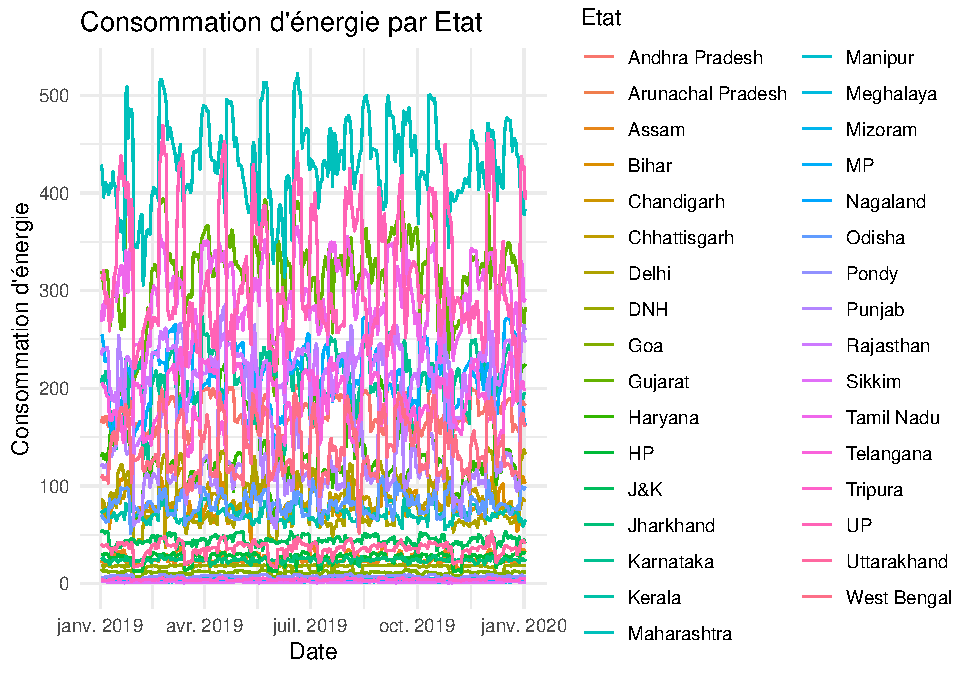
\includegraphics{Projet_CHESNAIS_GUIBERT_files/figure-latex/unnamed-chunk-9-1.pdf}

Ce graphique nous montre que nos données sont très irrégulières.
Cependant, la lecture des valeurs est assez compliqué à cause du nombre
important d'Etats et des fluctuations, c'est pourquoi la représentation
selon les régions d'Inde nous a paru pertinente.\\

{[}Représentation des données en différentes parties{]}.\{underline\}

Nous avons fixé des seuils par rapport à la moyenne de consommations des
Etats pour réaliser ces graphiques.

{[}Calcul de la moyenne par Etat{]}.\{underline\}

On calcule d'abord la moyenne par Etat et on ajoute cette moyenne a un
nouveau dataframe :

\begin{Shaded}
\begin{Highlighting}[]
\NormalTok{moyenne\_par\_etat }\OtherTok{\textless{}{-}} \FunctionTok{tapply}\NormalTok{(data}\SpecialCharTok{$}\NormalTok{Consommation, data}\SpecialCharTok{$}\NormalTok{Etat, mean)}
\NormalTok{moyenne\_par\_etat }\OtherTok{\textless{}{-}} \FunctionTok{data.frame}\NormalTok{(}\AttributeTok{Etat =} \FunctionTok{names}\NormalTok{(moyenne\_par\_etat), }
                               \AttributeTok{Moyenne =}\NormalTok{ moyenne\_par\_etat)}

\NormalTok{data\_complete }\OtherTok{\textless{}{-}} \FunctionTok{merge}\NormalTok{(data,moyenne\_par\_etat, }\AttributeTok{by =} \StringTok{"Etat"}\NormalTok{) }
\CommentTok{\# knitr::kable(data\_complete, caption = " Tableau des données avec la moyenne des consommations par Etat")}
\end{Highlighting}
\end{Shaded}

{[}Séparation de notre jeu de données{]}.\{underline\}

On sépare les données en 3 catégories d'Etats caractérisant leur
consommation d'énergie :

\begin{Shaded}
\begin{Highlighting}[]
\NormalTok{data\_inf }\OtherTok{\textless{}{-}}\NormalTok{ data\_complete }\SpecialCharTok{|\textgreater{}} 
  \FunctionTok{filter}\NormalTok{(Moyenne }\SpecialCharTok{\textless{}=} \DecValTok{50}\NormalTok{)}
\CommentTok{\# data\_inf}

\NormalTok{data\_moy }\OtherTok{\textless{}{-}}\NormalTok{ data\_complete }\SpecialCharTok{|\textgreater{}} 
  \FunctionTok{filter}\NormalTok{(Moyenne }\SpecialCharTok{\textgreater{}} \DecValTok{50} \SpecialCharTok{\&}\NormalTok{ Moyenne }\SpecialCharTok{\textless{}} \DecValTok{200}\NormalTok{)}
\CommentTok{\# data\_moy}

\NormalTok{data\_sup }\OtherTok{\textless{}{-}}\NormalTok{ data\_complete }\SpecialCharTok{|\textgreater{}} 
  \FunctionTok{filter}\NormalTok{(Moyenne }\SpecialCharTok{\textgreater{}=} \DecValTok{200}\NormalTok{)}
\CommentTok{\# data\_sup}
\end{Highlighting}
\end{Shaded}

{[}Représentations graphiques{]}.\{underline\}

\begin{Shaded}
\begin{Highlighting}[]
\FunctionTok{ggplot}\NormalTok{(data\_inf, }\FunctionTok{aes}\NormalTok{(}\AttributeTok{x =}\NormalTok{ Date, }\AttributeTok{y =}\NormalTok{ Consommation, }\AttributeTok{color =}\NormalTok{ Etat)) }\SpecialCharTok{+}
  \FunctionTok{geom\_line}\NormalTok{() }\SpecialCharTok{+}
  \FunctionTok{labs}\NormalTok{(}\AttributeTok{x =} \StringTok{"Date"}\NormalTok{, }\AttributeTok{y =} \StringTok{"Consommation d\textquotesingle{}énergie"}\NormalTok{, }
       \AttributeTok{title =} \StringTok{"Consommation d\textquotesingle{}énergie par Etat"}\NormalTok{, }
       \AttributeTok{subtitle =} \StringTok{"Etats consommant moins de 50 Mega Units en moyenne"}\NormalTok{) }\SpecialCharTok{+}
  \FunctionTok{theme\_minimal}\NormalTok{()}
\end{Highlighting}
\end{Shaded}

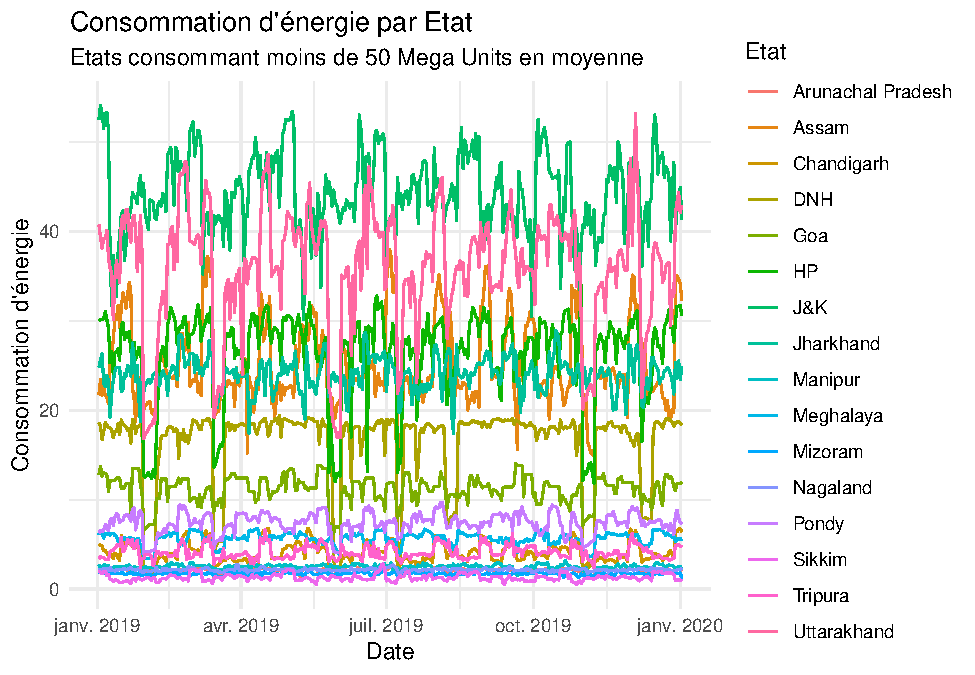
\includegraphics{Projet_CHESNAIS_GUIBERT_files/figure-latex/unnamed-chunk-12-1.pdf}

\begin{Shaded}
\begin{Highlighting}[]
\FunctionTok{ggplot}\NormalTok{(data\_moy, }\FunctionTok{aes}\NormalTok{(}\AttributeTok{x =}\NormalTok{ Date, }\AttributeTok{y =}\NormalTok{ Consommation, }\AttributeTok{color =}\NormalTok{ Etat)) }\SpecialCharTok{+}
  \FunctionTok{geom\_line}\NormalTok{() }\SpecialCharTok{+}
  \FunctionTok{labs}\NormalTok{(}\AttributeTok{x =} \StringTok{"Date"}\NormalTok{, }\AttributeTok{y =} \StringTok{"Consommation d\textquotesingle{}énergie"}\NormalTok{, }
       \AttributeTok{title =} \StringTok{"Consommation d\textquotesingle{}énergie par Etat"}\NormalTok{, }
       \AttributeTok{subtitle =} \StringTok{"Etats consommant entre 50 et 200 Mega Units en moyenne"}\NormalTok{) }\SpecialCharTok{+}
  \FunctionTok{theme\_minimal}\NormalTok{()}
\end{Highlighting}
\end{Shaded}

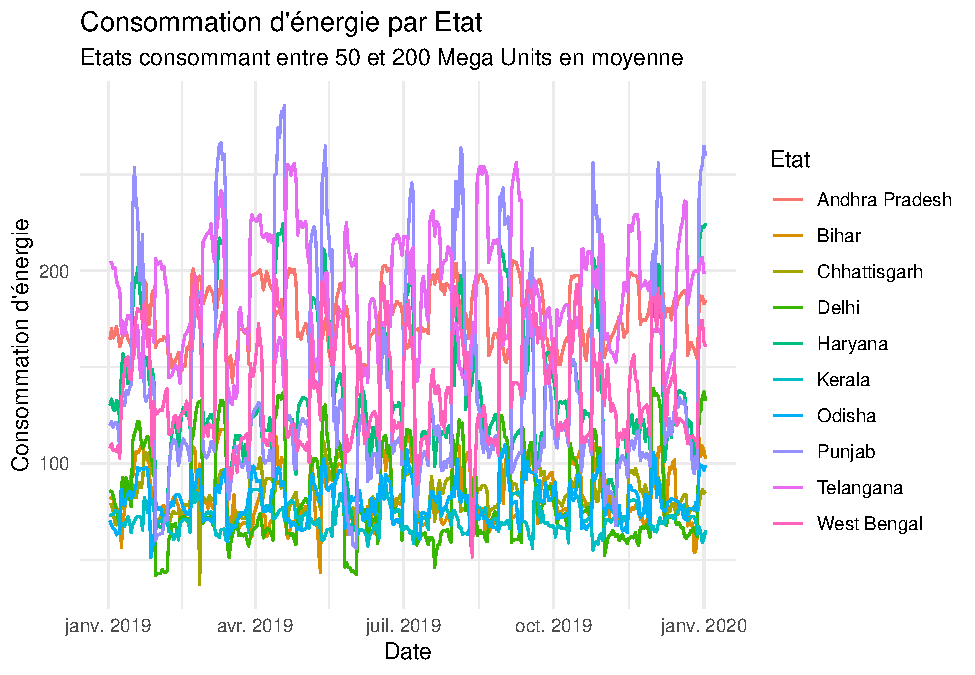
\includegraphics{Projet_CHESNAIS_GUIBERT_files/figure-latex/unnamed-chunk-12-2.pdf}

\begin{Shaded}
\begin{Highlighting}[]
\FunctionTok{ggplot}\NormalTok{(data\_sup, }\FunctionTok{aes}\NormalTok{(}\AttributeTok{x =}\NormalTok{ Date, }\AttributeTok{y =}\NormalTok{ Consommation, }\AttributeTok{color =}\NormalTok{ Etat)) }\SpecialCharTok{+}
  \FunctionTok{geom\_line}\NormalTok{() }\SpecialCharTok{+}
  \FunctionTok{labs}\NormalTok{(}\AttributeTok{x =} \StringTok{"Date"}\NormalTok{, }\AttributeTok{y =} \StringTok{"Consommation d\textquotesingle{}énergie"}\NormalTok{,}
       \AttributeTok{title =} \StringTok{"Consommation d\textquotesingle{}énergie par Etat"}\NormalTok{, }
       \AttributeTok{subtitle =} \StringTok{"Etats consommant plus de 200 Mega Units en moyenne"}\NormalTok{) }\SpecialCharTok{+}
  \FunctionTok{theme\_minimal}\NormalTok{()}
\end{Highlighting}
\end{Shaded}

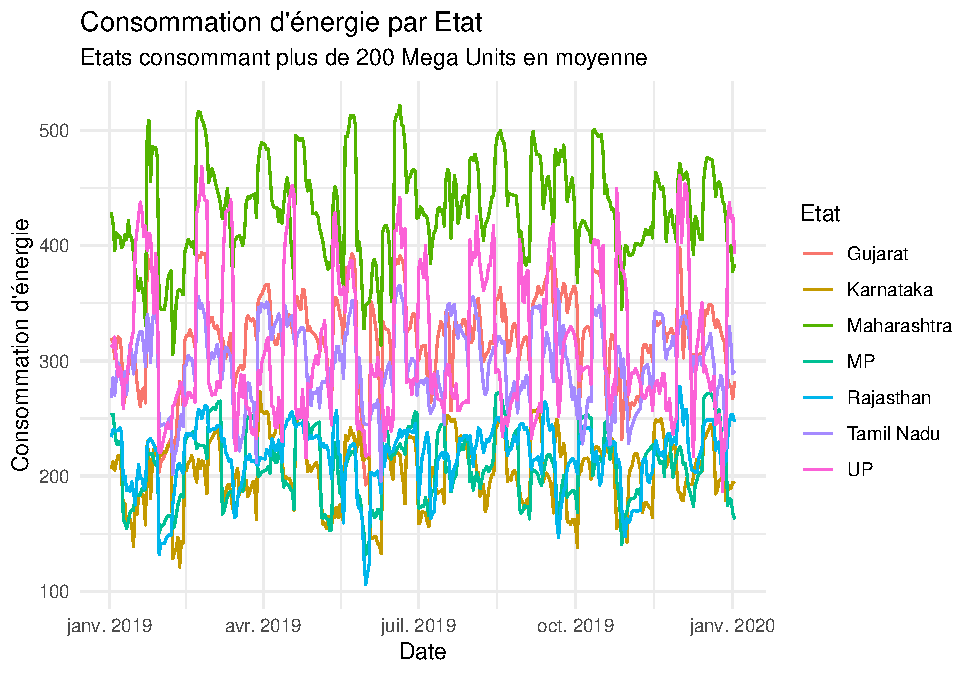
\includegraphics{Projet_CHESNAIS_GUIBERT_files/figure-latex/unnamed-chunk-12-3.pdf}

Grâce à ces représentations, il est plus facile d'observer et d'étudier
l'allure de nos données.\\

Pour la plupart des Etats, leur consommation varie beaucoup tout au long
de l'année, et, en quelques jours leur consommation peut doubler ou bien
diminuer subitement.

Cependant certains Etats comme le Tripura possède une consommation très
faible, et peu de variations dans son signal sont observées :

\begin{Shaded}
\begin{Highlighting}[]
\NormalTok{data }\SpecialCharTok{|\textgreater{}} 
  \FunctionTok{filter}\NormalTok{(Etat}\SpecialCharTok{==}\StringTok{"Tripura"}\NormalTok{) }\SpecialCharTok{|\textgreater{}} 
  \FunctionTok{ggplot}\NormalTok{(}\FunctionTok{aes}\NormalTok{(}\AttributeTok{x =}\NormalTok{ Date, }\AttributeTok{y =}\NormalTok{ Consommation)) }\SpecialCharTok{+}
  \FunctionTok{geom\_line}\NormalTok{() }\SpecialCharTok{+}
  \FunctionTok{labs}\NormalTok{(}\AttributeTok{x =} \StringTok{"Date"}\NormalTok{, }\AttributeTok{y =} \StringTok{"Consommation d\textquotesingle{}énergie"}\NormalTok{, }
       \AttributeTok{title =} \StringTok{"Consommation d\textquotesingle{}énergie du Tripura"}\NormalTok{) }\SpecialCharTok{+}
  \FunctionTok{theme\_minimal}\NormalTok{()}
\end{Highlighting}
\end{Shaded}

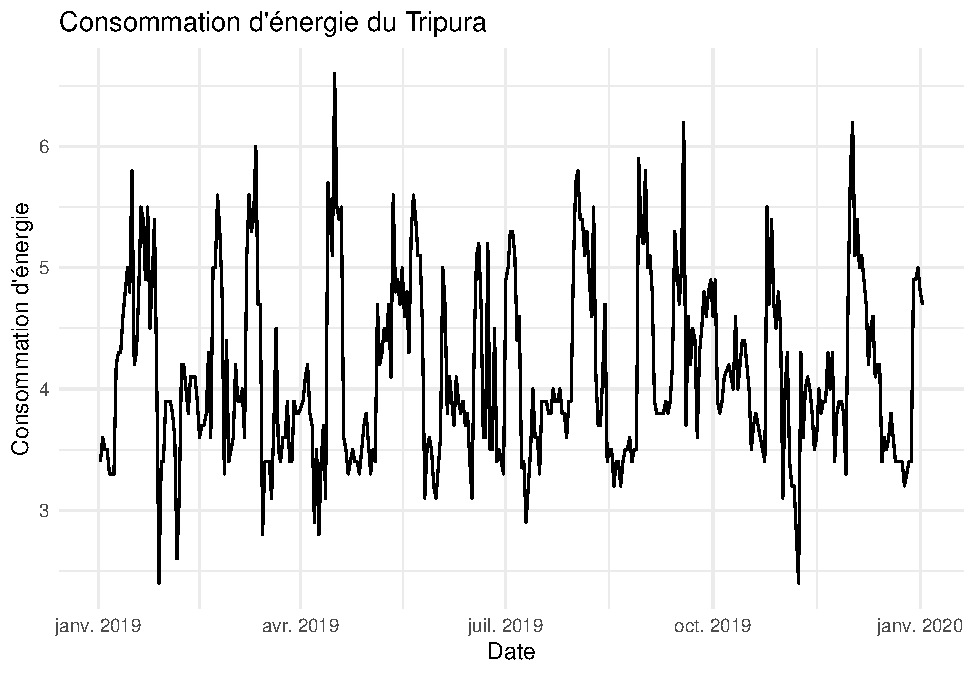
\includegraphics{Projet_CHESNAIS_GUIBERT_files/figure-latex/unnamed-chunk-13-1.pdf}

Sa consommation varie entre 2.4 et 6.6 mega Units.

\begin{Shaded}
\begin{Highlighting}[]
\FunctionTok{min}\NormalTok{(data}\SpecialCharTok{$}\NormalTok{Consommation[data}\SpecialCharTok{$}\NormalTok{Etat}\SpecialCharTok{==}\StringTok{"Tripura"}\NormalTok{])}
\end{Highlighting}
\end{Shaded}

\begin{verbatim}
## [1] 2.4
\end{verbatim}

\begin{Shaded}
\begin{Highlighting}[]
\FunctionTok{max}\NormalTok{(data}\SpecialCharTok{$}\NormalTok{Consommation[data}\SpecialCharTok{$}\NormalTok{Etat}\SpecialCharTok{==}\StringTok{"Tripura"}\NormalTok{])}
\end{Highlighting}
\end{Shaded}

\begin{verbatim}
## [1] 6.6
\end{verbatim}

A l'opposition du Punjab qui lui possède une très grande variation dans
sa consommation :

\begin{Shaded}
\begin{Highlighting}[]
\NormalTok{data }\SpecialCharTok{|\textgreater{}} 
  \FunctionTok{filter}\NormalTok{(Etat}\SpecialCharTok{==}\StringTok{"Punjab"}\NormalTok{) }\SpecialCharTok{|\textgreater{}} 
  \FunctionTok{ggplot}\NormalTok{(}\FunctionTok{aes}\NormalTok{(}\AttributeTok{x =}\NormalTok{ Date, }\AttributeTok{y =}\NormalTok{ Consommation)) }\SpecialCharTok{+}
  \FunctionTok{geom\_line}\NormalTok{() }\SpecialCharTok{+}
  \FunctionTok{labs}\NormalTok{(}\AttributeTok{x =} \StringTok{"Date"}\NormalTok{, }\AttributeTok{y =} \StringTok{"Consommation d\textquotesingle{}énergie"}\NormalTok{, }
       \AttributeTok{title =} \StringTok{"Consommation d\textquotesingle{}énergie du Punjab"}\NormalTok{) }\SpecialCharTok{+}
  \FunctionTok{theme\_minimal}\NormalTok{()}
\end{Highlighting}
\end{Shaded}

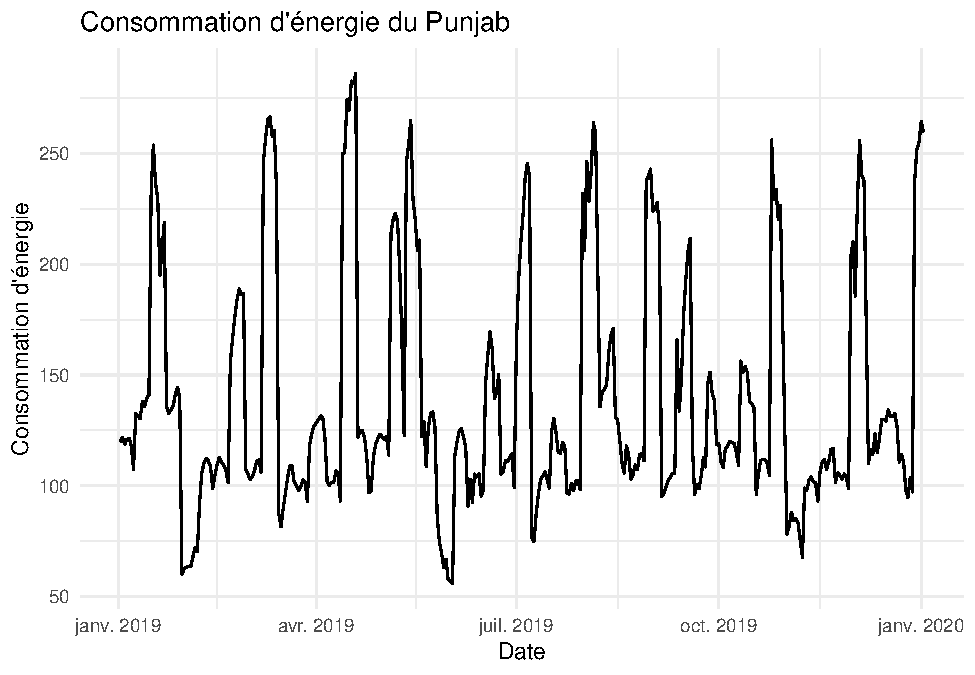
\includegraphics{Projet_CHESNAIS_GUIBERT_files/figure-latex/unnamed-chunk-15-1.pdf}

\begin{Shaded}
\begin{Highlighting}[]
\FunctionTok{min}\NormalTok{(data}\SpecialCharTok{$}\NormalTok{Consommation[data}\SpecialCharTok{$}\NormalTok{Etat}\SpecialCharTok{==}\StringTok{"Punjab"}\NormalTok{])}
\end{Highlighting}
\end{Shaded}

\begin{verbatim}
## [1] 56.1
\end{verbatim}

\begin{Shaded}
\begin{Highlighting}[]
\FunctionTok{max}\NormalTok{(data}\SpecialCharTok{$}\NormalTok{Consommation[data}\SpecialCharTok{$}\NormalTok{Etat}\SpecialCharTok{==}\StringTok{"Punjab"}\NormalTok{])}
\end{Highlighting}
\end{Shaded}

\begin{verbatim}
## [1] 286
\end{verbatim}

\uline{Tableau des moyennes de consommation par Etat}

\begin{Shaded}
\begin{Highlighting}[]
\NormalTok{knitr}\SpecialCharTok{::}\FunctionTok{kable}\NormalTok{(}\FunctionTok{tapply}\NormalTok{(data}\SpecialCharTok{$}\NormalTok{Consommation, data}\SpecialCharTok{$}\NormalTok{Etat, mean),}
             \StringTok{"simple"}\NormalTok{,}
             \AttributeTok{caption =} \StringTok{"Tableau des moyennes des consommation par Etat"}\NormalTok{,}
             \AttributeTok{col.names =} \StringTok{"Moyenne"}\NormalTok{,}
             \AttributeTok{longtable =} \ConstantTok{TRUE}\NormalTok{, }\AttributeTok{width =} \StringTok{"100\%"}\NormalTok{)}
\end{Highlighting}
\end{Shaded}

\begin{longtable}[]{@{}lr@{}}
\caption{Tableau des moyennes des consommation par Etat}\tabularnewline
\toprule()
& Moyenne \\
\midrule()
\endfirsthead
\toprule()
& Moyenne \\
\midrule()
\endhead
Andhra Pradesh & 175.891573 \\
Arunachal Pradesh & 2.108146 \\
Assam & 25.156601 \\
Bihar & 83.878652 \\
Chandigarh & 4.132584 \\
Chhattisgarh & 84.220646 \\
Delhi & 82.659831 \\
DNH & 16.415590 \\
Goa & 11.183427 \\
Gujarat & 321.564747 \\
Haryana & 137.518258 \\
HP & 26.582303 \\
J\&K & 44.331180 \\
Jharkhand & 23.998596 \\
Karnataka & 203.602247 \\
Kerala & 71.824298 \\
Maharashtra & 431.561517 \\
Manipur & 2.494101 \\
Meghalaya & 5.635674 \\
Mizoram & 1.712500 \\
MP & 208.722331 \\
Nagaland & 2.167416 \\
Odisha & 80.974438 \\
Pondy & 7.407865 \\
Punjab & 139.669522 \\
Rajasthan & 218.367977 \\
Sikkim & 1.296348 \\
Tamil Nadu & 297.655758 \\
Telangana & 188.360534 \\
Tripura & 4.145084 \\
UP & 314.962781 \\
Uttarakhand & 36.104494 \\
West Bengal & 139.527107 \\
\bottomrule()
\end{longtable}

\uline{Représentation selon la région}

L'Inde est divisée en 5 régions : le Nord (NR), Nord-Est (NER), le Sud
(SR), l'Est (ER) et l'Ouest (WR) Nous allons tracer les consommations en
fonction des régions (une couleur par région)./ De la même manière que
les représentations précédentes, nous ne pouvons représenter les régions
sur le même graphique. Sans diviser la représentation, il est difficile
de bien observer les différences entre les régions.

Nous décidons donc de représenter une région par graphique :

\begin{Shaded}
\begin{Highlighting}[]
\NormalTok{data }\SpecialCharTok{|\textgreater{}} 
  \FunctionTok{filter}\NormalTok{(Regions}\SpecialCharTok{==}\StringTok{"ER"}\NormalTok{) }\SpecialCharTok{|\textgreater{}} 
  \FunctionTok{ggplot}\NormalTok{(}\FunctionTok{aes}\NormalTok{(}\AttributeTok{x =}\NormalTok{ Date, }\AttributeTok{y =}\NormalTok{ Consommation,}\AttributeTok{color =}\NormalTok{ Etat)) }\SpecialCharTok{+}
  \FunctionTok{geom\_line}\NormalTok{() }\SpecialCharTok{+}
  \FunctionTok{labs}\NormalTok{(}\AttributeTok{x =} \StringTok{"Date"}\NormalTok{, }\AttributeTok{y =} \StringTok{"Consommation d\textquotesingle{}énergie"}\NormalTok{,}
       \AttributeTok{title =} \StringTok{"Consommation d\textquotesingle{}énergie pour les Etats de l\textquotesingle{}Est de l\textquotesingle{}Inde"}\NormalTok{) }\SpecialCharTok{+}
  \FunctionTok{theme\_minimal}\NormalTok{()}
\end{Highlighting}
\end{Shaded}

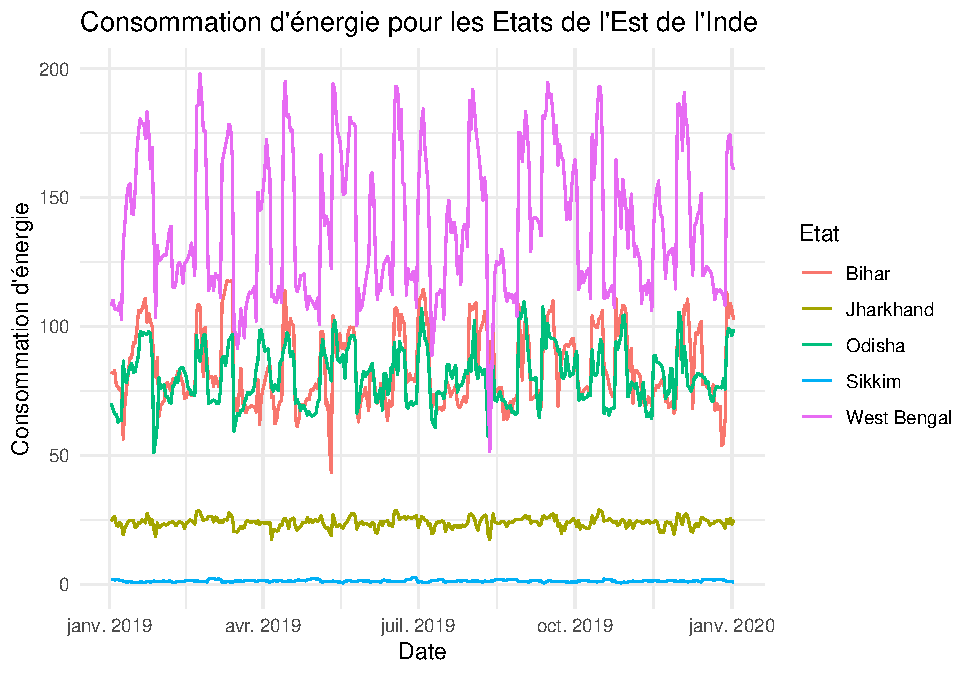
\includegraphics{Projet_CHESNAIS_GUIBERT_files/figure-latex/unnamed-chunk-17-1.pdf}

\begin{Shaded}
\begin{Highlighting}[]
\NormalTok{data }\SpecialCharTok{|\textgreater{}} 
  \FunctionTok{filter}\NormalTok{(Regions}\SpecialCharTok{==}\StringTok{"NER"}\NormalTok{) }\SpecialCharTok{|\textgreater{}} 
  \FunctionTok{ggplot}\NormalTok{(}\FunctionTok{aes}\NormalTok{(}\AttributeTok{x =}\NormalTok{ Date, }\AttributeTok{y =}\NormalTok{ Consommation,}\AttributeTok{color =}\NormalTok{ Etat)) }\SpecialCharTok{+}
  \FunctionTok{geom\_line}\NormalTok{() }\SpecialCharTok{+}
  \FunctionTok{labs}\NormalTok{(}\AttributeTok{x =} \StringTok{"Date"}\NormalTok{, }\AttributeTok{y =} \StringTok{"Consommation d\textquotesingle{}énergie"}\NormalTok{, }
       \AttributeTok{title =} \StringTok{"Consommation d\textquotesingle{}énergie pour les Etats du Nord Est de l\textquotesingle{}Inde"}\NormalTok{) }\SpecialCharTok{+}
  \FunctionTok{theme\_minimal}\NormalTok{()}
\end{Highlighting}
\end{Shaded}

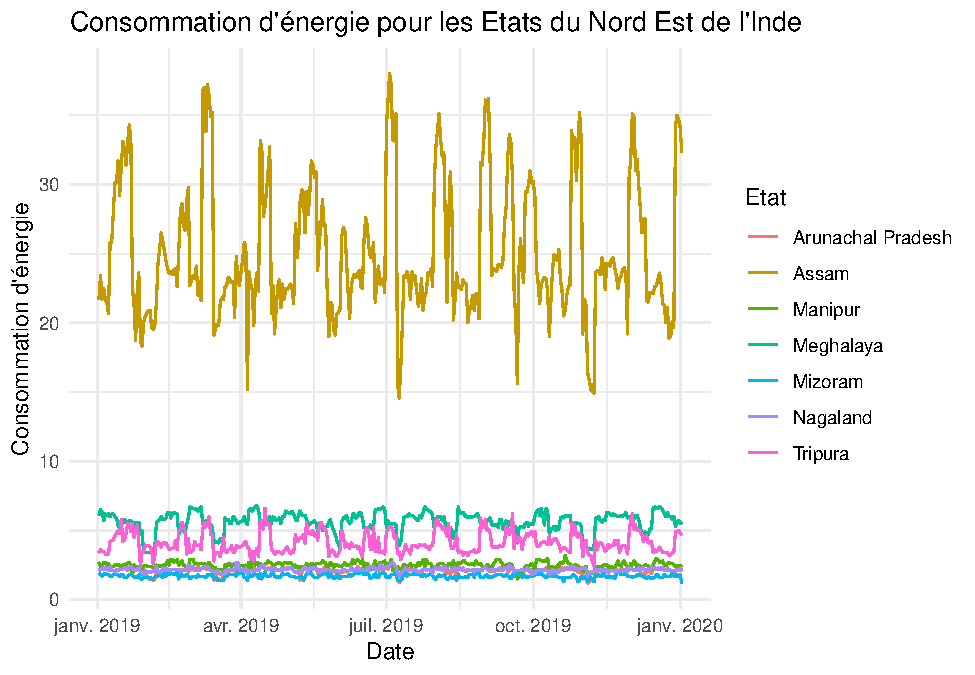
\includegraphics{Projet_CHESNAIS_GUIBERT_files/figure-latex/unnamed-chunk-17-2.pdf}

\begin{Shaded}
\begin{Highlighting}[]
\NormalTok{data }\SpecialCharTok{|\textgreater{}} 
  \FunctionTok{filter}\NormalTok{(Regions}\SpecialCharTok{==}\StringTok{"NR"}\NormalTok{) }\SpecialCharTok{|\textgreater{}} 
  \FunctionTok{ggplot}\NormalTok{(}\FunctionTok{aes}\NormalTok{(}\AttributeTok{x =}\NormalTok{ Date, }\AttributeTok{y =}\NormalTok{ Consommation,}\AttributeTok{color =}\NormalTok{ Etat)) }\SpecialCharTok{+}
  \FunctionTok{geom\_line}\NormalTok{() }\SpecialCharTok{+}
  \FunctionTok{labs}\NormalTok{(}\AttributeTok{x =} \StringTok{"Date"}\NormalTok{, }\AttributeTok{y =} \StringTok{"Consommation d\textquotesingle{}énergie"}\NormalTok{, }
       \AttributeTok{title =} \StringTok{"Consommation d\textquotesingle{}énergie pour les Etats du Nord de l\textquotesingle{}Inde"}\NormalTok{) }\SpecialCharTok{+}
  \FunctionTok{theme\_minimal}\NormalTok{()}
\end{Highlighting}
\end{Shaded}

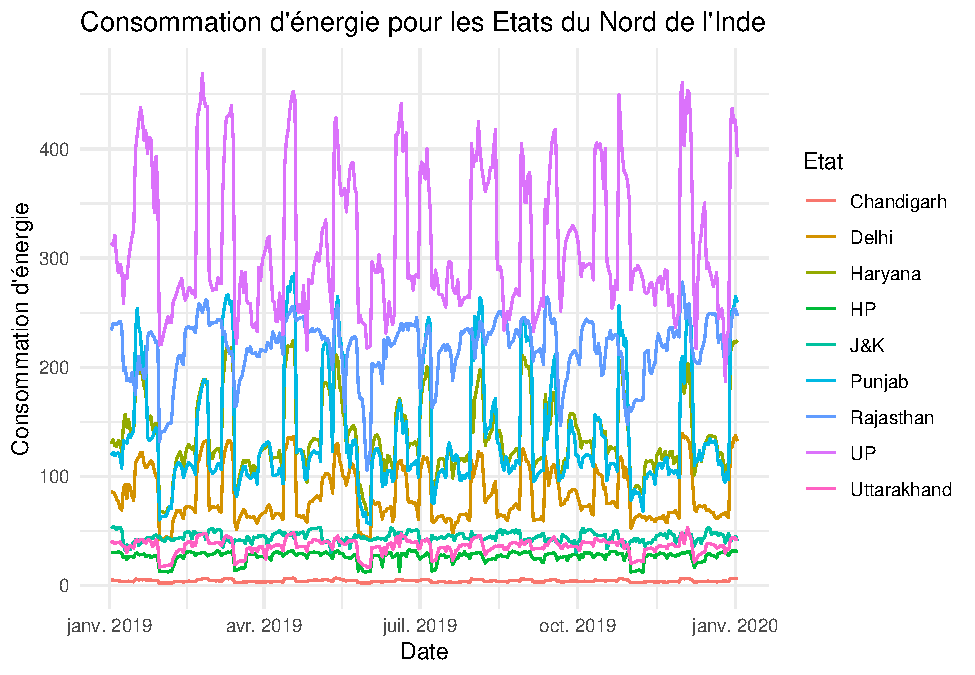
\includegraphics{Projet_CHESNAIS_GUIBERT_files/figure-latex/unnamed-chunk-17-3.pdf}

\begin{Shaded}
\begin{Highlighting}[]
\NormalTok{data }\SpecialCharTok{|\textgreater{}} 
  \FunctionTok{filter}\NormalTok{(Regions}\SpecialCharTok{==}\StringTok{"SR"}\NormalTok{) }\SpecialCharTok{|\textgreater{}} 
  \FunctionTok{ggplot}\NormalTok{(}\FunctionTok{aes}\NormalTok{(}\AttributeTok{x =}\NormalTok{ Date, }\AttributeTok{y =}\NormalTok{ Consommation,}\AttributeTok{color =}\NormalTok{ Etat)) }\SpecialCharTok{+}
  \FunctionTok{geom\_line}\NormalTok{() }\SpecialCharTok{+}
  \FunctionTok{labs}\NormalTok{(}\AttributeTok{x =} \StringTok{"Date"}\NormalTok{, }\AttributeTok{y =} \StringTok{"Consommation d\textquotesingle{}énergie"}\NormalTok{, }
       \AttributeTok{title =} \StringTok{"Consommation d\textquotesingle{}énergie pour les Etats du Sud de l\textquotesingle{}Inde"}\NormalTok{) }\SpecialCharTok{+}
  \FunctionTok{theme\_minimal}\NormalTok{()}
\end{Highlighting}
\end{Shaded}

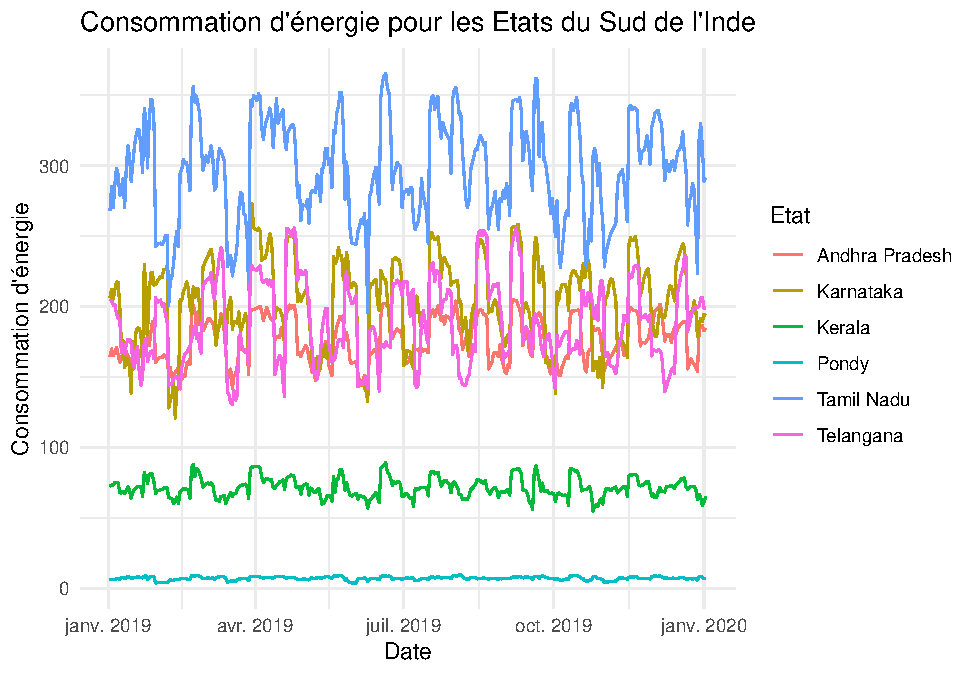
\includegraphics{Projet_CHESNAIS_GUIBERT_files/figure-latex/unnamed-chunk-17-4.pdf}

\begin{Shaded}
\begin{Highlighting}[]
\NormalTok{data }\SpecialCharTok{|\textgreater{}} 
  \FunctionTok{filter}\NormalTok{(Regions}\SpecialCharTok{==}\StringTok{"WR"}\NormalTok{) }\SpecialCharTok{|\textgreater{}} 
  \FunctionTok{ggplot}\NormalTok{(}\FunctionTok{aes}\NormalTok{(}\AttributeTok{x =}\NormalTok{ Date, }\AttributeTok{y =}\NormalTok{ Consommation,}\AttributeTok{color =}\NormalTok{ Etat)) }\SpecialCharTok{+}
  \FunctionTok{geom\_line}\NormalTok{() }\SpecialCharTok{+}
  \FunctionTok{labs}\NormalTok{(}\AttributeTok{x =} \StringTok{"Date"}\NormalTok{, }\AttributeTok{y =} \StringTok{"Consommation d\textquotesingle{}énergie"}\NormalTok{, }
       \AttributeTok{title =} \StringTok{"Consommation d\textquotesingle{}énergie pour les Etats de l\textquotesingle{}Ouest de l\textquotesingle{}Inde"}\NormalTok{) }\SpecialCharTok{+}
  \FunctionTok{theme\_minimal}\NormalTok{()}
\end{Highlighting}
\end{Shaded}

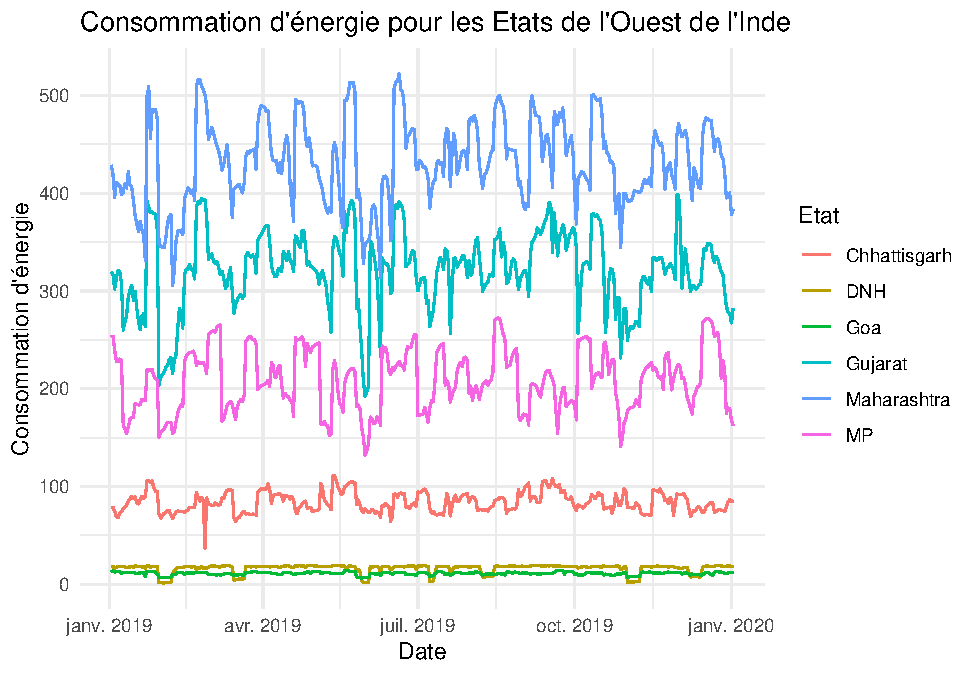
\includegraphics{Projet_CHESNAIS_GUIBERT_files/figure-latex/unnamed-chunk-17-5.pdf}

Au sein de chaque région de l'Inde, nous observons de forts contrastes
de consommation d'énergie. Nous pouvons noter une différence d'échelle
entre les graphiques. Par exemple, dans le Sud de l'Inde, Pondy a une
faible consommation d'énergie (entre 4 et 10 Mega Units) à l'opposé de
Tamil Nadu où celle-ci varie entre 200 et 370 Mega Units.

Il serait intéressant de consulter l'avis d'un économiste ou politicien
pour analyser et comprendre ces grandes disparités au sein des régions
de l'Inde.

Nous construisons le tableau des moyennes de consommation par région :

\begin{Shaded}
\begin{Highlighting}[]
\NormalTok{knitr}\SpecialCharTok{::}\FunctionTok{kable}\NormalTok{(}\FunctionTok{tapply}\NormalTok{(data}\SpecialCharTok{$}\NormalTok{Consommation, data}\SpecialCharTok{$}\NormalTok{Regions, mean),}
             \StringTok{"simple"}\NormalTok{, }\AttributeTok{col.names =} \StringTok{"moyenne"}\NormalTok{, }
             \AttributeTok{caption =} \StringTok{"Tableau des moyennes des consommation d\textquotesingle{}énergie par région"}\NormalTok{,}
             \AttributeTok{longtable =} \ConstantTok{TRUE}\NormalTok{, }\AttributeTok{width =} \StringTok{"100\%"}\NormalTok{)}
\end{Highlighting}
\end{Shaded}

\begin{longtable}[]{@{}lr@{}}
\caption{Tableau des moyennes des consommation d'énergie par
région}\tabularnewline
\toprule()
& moyenne \\
\midrule()
\endfirsthead
\toprule()
& moyenne \\
\midrule()
\endhead
ER & 65.935028 \\
NER & 6.202789 \\
NR & 111.592104 \\
SR & 157.457046 \\
WR & 178.944710 \\
\bottomrule()
\end{longtable}

Nous observons une hétérogénéité en termes de consommations entre les
régions de l'Inde. En effet, le Nord-Est a une consommation très faible
par rapport à l'Ouest. Peut-être qu'un expert pourrait aussi nous donner
les causes de ces écarts de consommation.

\hypertarget{ii.-ondelettes}{%
\section{II. Ondelettes}\label{ii.-ondelettes}}

Puisque nos signaux sont irréguliers, notre choix de lissage s'est
d'abord tourné vers les ondelettes car elles ont des bonnes propriétés
de compressions et sont adaptées à ce type de données.

Pour pouvoir poursuivre cette étude, nous avons du transformer notre
dataframe de départ pour avoir chaque Etat en colonne avec la valeur de
consommation en ligne pour chaque point de mesure.

\begin{Shaded}
\begin{Highlighting}[]
\NormalTok{data\_long }\OtherTok{\textless{}{-}} \FunctionTok{data.frame}\NormalTok{(}\StringTok{"Etat"} \OtherTok{=}\NormalTok{ data}\SpecialCharTok{$}\NormalTok{Etat,}
                        \StringTok{"Date"}\OtherTok{=}\NormalTok{ data}\SpecialCharTok{$}\NormalTok{Date,}\StringTok{"Consommation"} \OtherTok{=}\NormalTok{ data}\SpecialCharTok{$}\NormalTok{Consommation)}

\NormalTok{data\_long }\OtherTok{\textless{}{-}}\NormalTok{ data\_long }\SpecialCharTok{|\textgreater{}} 
\NormalTok{  tidyr}\SpecialCharTok{::}\FunctionTok{pivot\_wider}\NormalTok{(}\AttributeTok{names\_from =} \StringTok{"Etat"}\NormalTok{, }\AttributeTok{values\_from =} \StringTok{"Consommation"}\NormalTok{)}

\NormalTok{data\_long }\OtherTok{\textless{}{-}} \FunctionTok{as.data.frame}\NormalTok{(data\_long)}
\FunctionTok{head}\NormalTok{(data\_long)}
\end{Highlighting}
\end{Shaded}

\begin{verbatim}
##         Date Punjab Haryana Rajasthan Delhi    UP Uttarakhand   HP  J&K
## 1 2019-01-02  119.9   130.3     234.1  85.8 313.9        40.7 30.0 52.5
## 2 2019-01-03  121.9   133.5     240.2  85.5 311.8        39.3 30.1 54.1
## 3 2019-01-04  118.8   128.2     239.8  83.5 320.7        38.1 30.1 53.2
## 4 2019-01-05  121.0   127.5     239.1  79.2 299.0        39.2 30.2 51.5
## 5 2019-01-06  121.4   132.6     240.4  76.6 286.8        39.2 31.0 53.2
## 6 2019-01-07  118.0   132.1     241.9  71.1 294.2        40.1 30.1 53.3
##   Chandigarh Chhattisgarh Gujarat    MP Maharashtra  Goa  DNH Andhra Pradesh
## 1        5.0         78.7   319.5 253.0       428.6 12.8 18.6          164.6
## 2        4.9         78.8   316.7 253.6       419.6 13.7 18.2          170.1
## 3        4.8         74.8   301.9 239.3       395.8 12.6 16.7          165.2
## 4        4.3         69.0   313.2 228.2       411.1 13.0 17.6          167.4
## 5        4.3         68.1   320.7 227.4       408.6 12.9 18.6          171.2
## 6        4.0         73.1   319.4 230.3       408.1 12.7 18.3          166.4
##   Telangana Karnataka Kerala Tamil Nadu Pondy Bihar Jharkhand Odisha
## 1     204.2     206.3   72.7      268.3   6.3  82.3      24.8   70.2
## 2     204.5     212.2   73.6      285.2   6.5  82.0      25.6   67.9
## 3     201.2     205.3   73.4      270.3   6.4  82.9      26.3   66.3
## 4     201.7     212.4   75.4      286.8   6.6  77.0      23.0   65.8
## 5     194.9     217.5   75.4      298.3   7.2  76.4      22.6   62.9
## 6     191.9     217.4   74.9      294.2   7.0  75.3      23.9   64.0
##   West Bengal Sikkim Arunachal Pradesh Assam Manipur Meghalaya Mizoram Nagaland
## 1       108.2    2.0               2.1  21.7     2.7       6.1     1.9      2.2
## 2       110.2    1.9               2.2  23.4     2.4       6.5     1.8      2.2
## 3       106.8    1.7               2.2  21.7     2.4       6.3     1.7      2.2
## 4       107.0    2.0               2.2  22.5     2.7       5.7     1.8      2.3
## 5       106.4    2.0               2.2  21.7     2.7       6.2     1.9      2.3
## 6       109.3    1.5               2.2  21.4     2.5       6.1     1.8      2.3
##   Tripura
## 1     3.4
## 2     3.6
## 3     3.5
## 4     3.5
## 5     3.3
## 6     3.3
\end{verbatim}

Le problème ici est que la longueur des courbes de consommation n'est
pas de la forme \(2^J\). Ces courbes sont de longueur 356, on symétrise
le signal à la fin pour atteindre une longueur de 512. On se ramènera à
la fin au signal de départ de taille 356.

Nous représentons le signal pour un Etat (ici le Punjab) :

\begin{Shaded}
\begin{Highlighting}[]
\NormalTok{i }\OtherTok{=} \DecValTok{2}
\NormalTok{y }\OtherTok{\textless{}{-}}\NormalTok{  data\_long[,i]}
\CommentTok{\# y}

\FunctionTok{plot}\NormalTok{(}\DecValTok{1}\SpecialCharTok{:}\DecValTok{356}\NormalTok{,y,}\AttributeTok{type=}\StringTok{"l"}\NormalTok{,}\AttributeTok{main=}\StringTok{"Signal de départ"}\NormalTok{, }\AttributeTok{ylab =} \StringTok{"Consommation"}\NormalTok{, }\AttributeTok{xlab=}\StringTok{"Jour"}\NormalTok{)}
\end{Highlighting}
\end{Shaded}

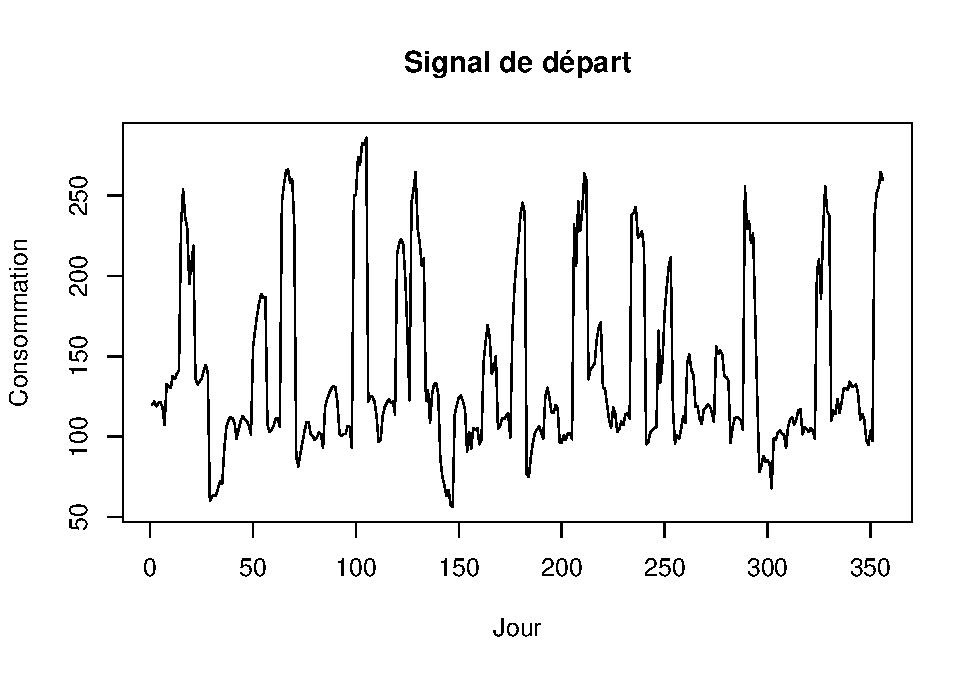
\includegraphics{Projet_CHESNAIS_GUIBERT_files/figure-latex/unnamed-chunk-20-1.pdf}

\begin{Shaded}
\begin{Highlighting}[]
\CommentTok{\# Créer un signal symétrisé}
\NormalTok{ysym }\OtherTok{=} \FunctionTok{c}\NormalTok{(y, }\FunctionTok{rev}\NormalTok{(}\FunctionTok{tail}\NormalTok{(y, }\AttributeTok{n=} \DecValTok{512}\SpecialCharTok{{-}}\FunctionTok{length}\NormalTok{(y)))) }\CommentTok{\# on choisit 512 pour avoir une puissance de 2}

\CommentTok{\# Tracer le signal symétrisé}
\FunctionTok{plot}\NormalTok{(ysym, }\AttributeTok{type =} \StringTok{"l"}\NormalTok{, }\AttributeTok{main =} \StringTok{"Signal symétrisé"}\NormalTok{, }
     \AttributeTok{ylab =} \StringTok{"Consommation"}\NormalTok{, }\AttributeTok{xlab =} \StringTok{"Jour"}\NormalTok{)}

\CommentTok{\# Ajouter une ligne verticale à la position}
\CommentTok{\# axe de symétrie : 361 jours}
\FunctionTok{abline}\NormalTok{(}\AttributeTok{v =} \DecValTok{356}\NormalTok{, }\AttributeTok{lty =} \DecValTok{2}\NormalTok{)}
\end{Highlighting}
\end{Shaded}

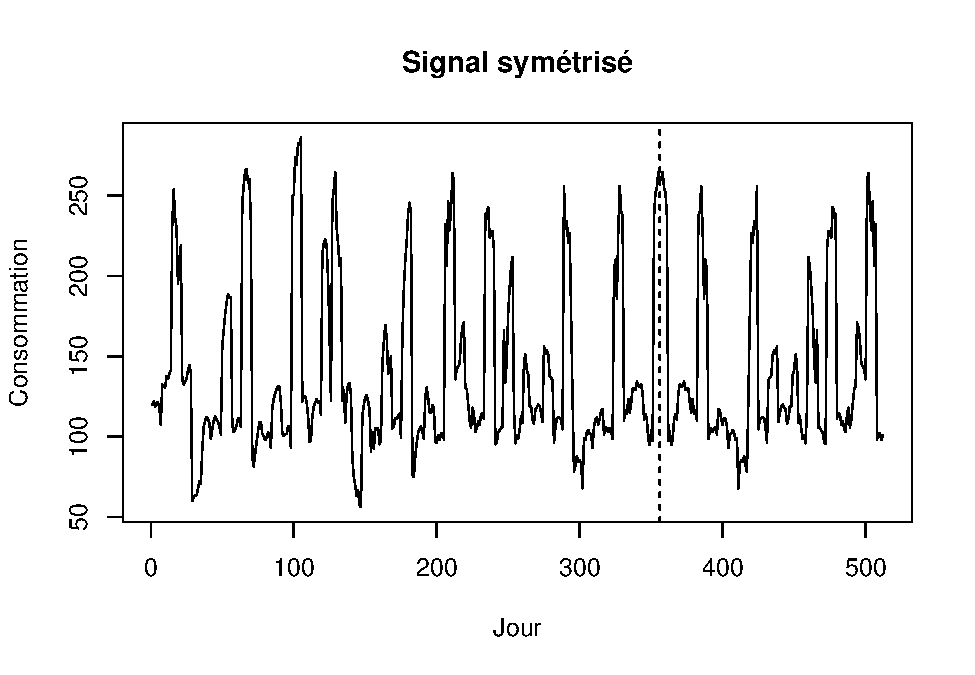
\includegraphics{Projet_CHESNAIS_GUIBERT_files/figure-latex/unnamed-chunk-20-2.pdf}

La méthode des ondelettes est complexe et nous ne disposons pas des
connaissances nécessaires pour faire une analyse très approndie. De
plus, il n'est pas possible de réaliser une ACP avec les ondelettes.

Nous nous tournons donc vers le lissage par moindres carrés pénalisés à
l'aide des bases de splines pour continuer notre étude.

\hypertarget{iii.-lissage-par-moindres-carruxe9s-puxe9nalisuxe9s---base-de-spline}{%
\section{III. Lissage par moindres carrés pénalisés - Base de
Spline}\label{iii.-lissage-par-moindres-carruxe9s-puxe9nalisuxe9s---base-de-spline}}

L'utilisation d'une base de spline pénalisée nous a semblé être adaptée
à nos signaux. Effectivement, cette méthode présente une grande
flexibilité de modélisation pour les données plus ou moins irrégulières.
Cette approche permet de capturer des comportements non linéaires, de
gérer les valeurs aberrantes, de réduire la dimension de l'espace des
caractéristiques, et de s'adapter à diverses structures de données. La
pénalisation va nous permet d'éviter un sur-ajustement de nos données.

\hypertarget{iii.a.-lissage-dune-trajectoire-pour-un-etat}{%
\subsection{III.A. Lissage d'une trajectoire (pour un
Etat)}\label{iii.a.-lissage-dune-trajectoire-pour-un-etat}}

Nous allons d'abotrd effectuer le lissage sur un seul Etat : le Punjab,
pour ensuite généraliser à l'ensemble des Etats.

\uline{Représentation de la consommation d'énergie}

\begin{Shaded}
\begin{Highlighting}[]
\NormalTok{i }\OtherTok{=} \DecValTok{2}
\NormalTok{y }\OtherTok{\textless{}{-}}\NormalTok{ data\_long[, }\DecValTok{2}\NormalTok{] }
\NormalTok{tps }\OtherTok{\textless{}{-}} \DecValTok{1}\SpecialCharTok{:}\DecValTok{356}
\FunctionTok{plot}\NormalTok{(tps,y,}\AttributeTok{type=}\StringTok{"l"}\NormalTok{, }\AttributeTok{main =} \StringTok{"Consommation d\textquotesingle{}énergie du Punjab"}\NormalTok{)}
\end{Highlighting}
\end{Shaded}

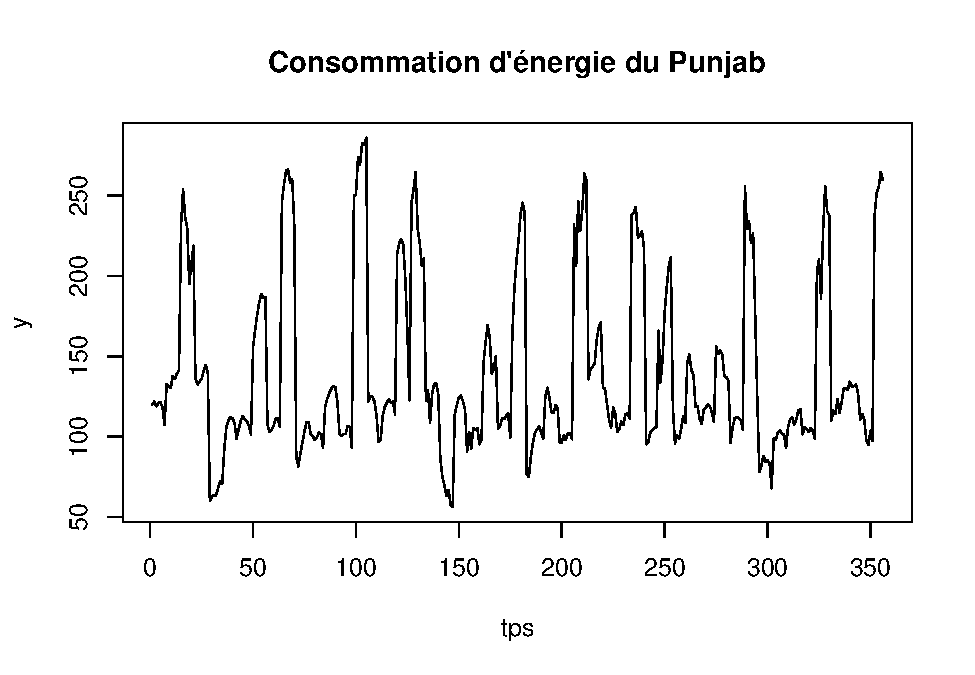
\includegraphics{Projet_CHESNAIS_GUIBERT_files/figure-latex/unnamed-chunk-21-1.pdf}

\uline{Lissage par moindres carrés pénalisés sur la première courbe}

\begin{Shaded}
\begin{Highlighting}[]
\NormalTok{splbasis }\OtherTok{=} \FunctionTok{create.bspline.basis}\NormalTok{(}\AttributeTok{rangeval =} \FunctionTok{c}\NormalTok{(}\DecValTok{1}\NormalTok{,}\DecValTok{356}\NormalTok{), }\CommentTok{\# 1 à 356 jours}
                                \AttributeTok{norder=}\DecValTok{6}\NormalTok{, }
                                \AttributeTok{breaks=}\FunctionTok{seq}\NormalTok{(}\DecValTok{1}\NormalTok{,}\DecValTok{356}\NormalTok{,}\AttributeTok{length=}\DecValTok{35}\NormalTok{))}
\CommentTok{\# définition une base de B{-}spline entre 1 et 356 (les dates) }
\CommentTok{\# ordre 6 }

\FunctionTok{plot}\NormalTok{(splbasis)}
\end{Highlighting}
\end{Shaded}

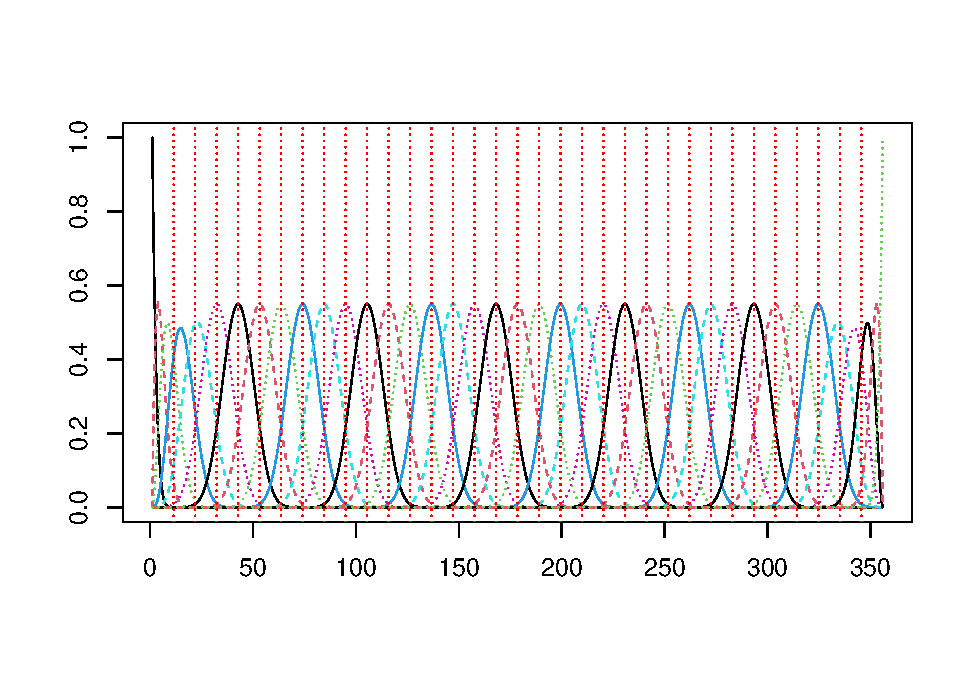
\includegraphics{Projet_CHESNAIS_GUIBERT_files/figure-latex/unnamed-chunk-22-1.pdf}

\begin{Shaded}
\begin{Highlighting}[]
\FunctionTok{summary}\NormalTok{(splbasis)}
\end{Highlighting}
\end{Shaded}

\begin{verbatim}
## 
## Basis object:
## 
##   Type:   bspline 
## 
##   Range:  1  to  356 
## 
##   Number of basis functions:  39
\end{verbatim}

Il s'agit d'une base de type ``bspline'' ce qui signifie qu'elle utilise
les fonctions B-splines pour modéliser les données. Dans cette base, il
y a 39 fonctions de base, utilisées pour construire la représentation
fonctionnelle des données.

La plage des données s'étend entre 1 et 356, correspondant à nos temps
de mesure.

Nous allons rechercher la valeur de lambda optimale pour trouver le
meilleur lissage de nos données.

\begin{Shaded}
\begin{Highlighting}[]
\NormalTok{i }\OtherTok{=} \DecValTok{2}
\NormalTok{y }\OtherTok{=}\NormalTok{ data\_long[,i]}
\NormalTok{gcv }\OtherTok{=} \DecValTok{1}\SpecialCharTok{:}\DecValTok{30} \CommentTok{\# grille de lambda}
\ControlFlowTok{for}\NormalTok{ (i }\ControlFlowTok{in} \DecValTok{1}\SpecialCharTok{:}\DecValTok{30}\NormalTok{)\{}
\NormalTok{  lambda }\OtherTok{=} \FunctionTok{exp}\NormalTok{(i}\DecValTok{{-}10}\NormalTok{) }
\NormalTok{  fdpar}\OtherTok{=} \FunctionTok{fdPar}\NormalTok{(splbasis,}\AttributeTok{Lfdobj =}\DecValTok{4}\NormalTok{,}\AttributeTok{lambda=}\NormalTok{lambda)}
\NormalTok{  smoothdata }\OtherTok{=} \FunctionTok{smooth.basis}\NormalTok{(tps,y,}\AttributeTok{fdParobj =}\NormalTok{ fdpar) }
\NormalTok{  gcv[i] }\OtherTok{=}\NormalTok{ smoothdata}\SpecialCharTok{$}\NormalTok{gcv }
\NormalTok{\}}
\FunctionTok{plot}\NormalTok{(gcv)}
\end{Highlighting}
\end{Shaded}

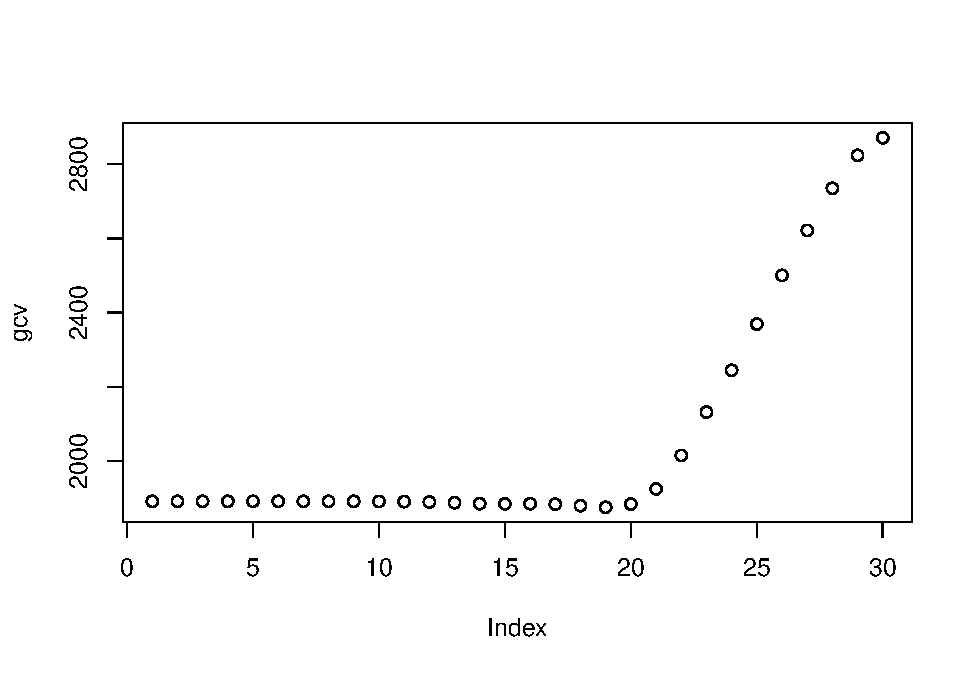
\includegraphics{Projet_CHESNAIS_GUIBERT_files/figure-latex/unnamed-chunk-24-1.pdf}

\begin{Shaded}
\begin{Highlighting}[]
\FunctionTok{which.min}\NormalTok{(gcv)}
\end{Highlighting}
\end{Shaded}

\begin{verbatim}
## [1] 19
\end{verbatim}

Nous obtenons une valeur de lambda égale à 19 pour l'Etat du Punjab.

Nous évaluons notre base de spline avec cette valeur optimale de lambda.

\begin{Shaded}
\begin{Highlighting}[]
\NormalTok{lambda }\OtherTok{=} \FunctionTok{exp}\NormalTok{(}\FunctionTok{which.min}\NormalTok{(gcv)}\SpecialCharTok{{-}}\DecValTok{10}\NormalTok{)}
\NormalTok{fdparTemp }\OtherTok{=} \FunctionTok{fdPar}\NormalTok{(splbasis,}\AttributeTok{Lfdobj =} \DecValTok{4}\NormalTok{,}\AttributeTok{lambda=}\NormalTok{lambda) }
\NormalTok{smoothdata }\OtherTok{=} \FunctionTok{smooth.basis}\NormalTok{(tps,y,}\AttributeTok{fdParobj =}\NormalTok{ fdpar)}
\end{Highlighting}
\end{Shaded}

Nous représentons sur un même graphe les observations et la fonction
estimée reconstruite ˆf.

\begin{Shaded}
\begin{Highlighting}[]
\FunctionTok{plotfit.fd}\NormalTok{(y,}\CommentTok{\# valeur de consommation pour un pays}
\NormalTok{           tps, }\CommentTok{\# les dates}
\NormalTok{           smoothdata}\SpecialCharTok{$}\NormalTok{fd, }\CommentTok{\# nos données estimées}
           \CommentTok{\# 1 à 356 }
           \AttributeTok{pch=}\DecValTok{20}\NormalTok{,}
           \AttributeTok{cex=}\FloatTok{0.5}\NormalTok{,}
           \AttributeTok{main=}\StringTok{"les observations et la fonction estimée }\SpecialCharTok{\textbackslash{}n}\StringTok{ reconstruite ˆf"}\NormalTok{,}
           \AttributeTok{ylab =} \StringTok{"consommation d\textquotesingle{}énergie"}\NormalTok{,}
           \AttributeTok{xlab=}\StringTok{"temps"}\NormalTok{)}
\end{Highlighting}
\end{Shaded}

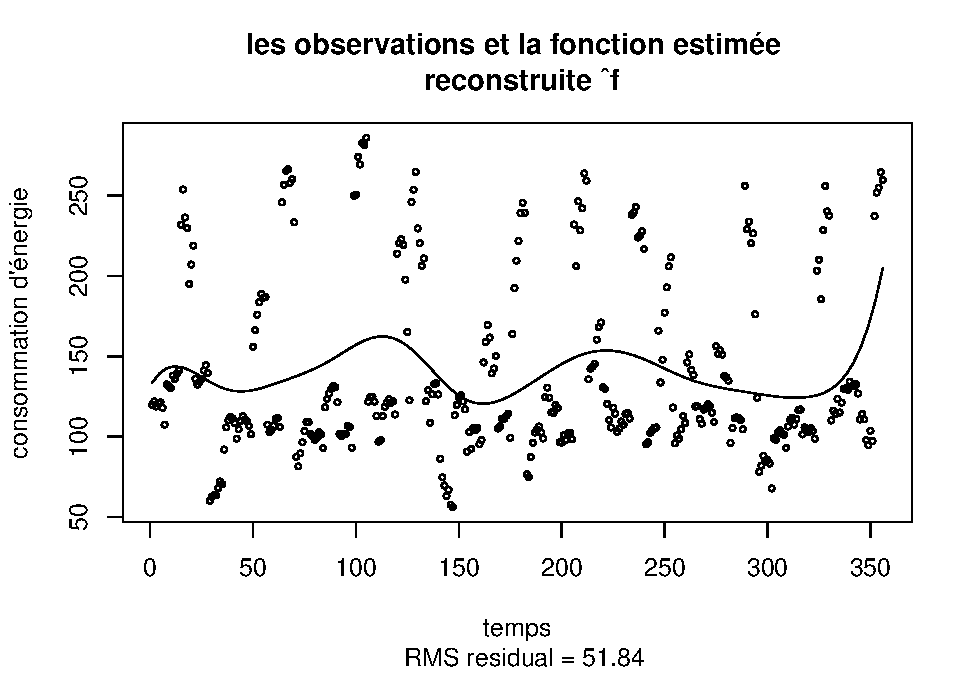
\includegraphics{Projet_CHESNAIS_GUIBERT_files/figure-latex/unnamed-chunk-26-1.pdf}

Nous obtenons une fonction estimée reconstruite lisse pour l'Etat du
Punjab. Elle est beaucoup moins irrégulière que nos données de base.
Elle prend globalement en compte les variations de consommation
d'énergie du Punjab sur une l'année 2019.

Nous représentons la dérivée première et la dérivée seconde sur le même
graphique :

\begin{Shaded}
\begin{Highlighting}[]
\NormalTok{fhatprim }\OtherTok{=} \FunctionTok{eval.fd}\NormalTok{(tps,smoothdata}\SpecialCharTok{$}\NormalTok{fd,}\AttributeTok{Lfdobj=}\DecValTok{1}\NormalTok{)}
\NormalTok{fhatpprim }\OtherTok{=} \FunctionTok{eval.fd}\NormalTok{(tps,smoothdata}\SpecialCharTok{$}\NormalTok{fd,}\AttributeTok{Lfdobj=}\DecValTok{2}\NormalTok{)}
\FunctionTok{matplot}\NormalTok{(tps,}\FunctionTok{cbind}\NormalTok{(fhatprim,fhatpprim),}\AttributeTok{type=}\StringTok{"l"}\NormalTok{)}
\end{Highlighting}
\end{Shaded}

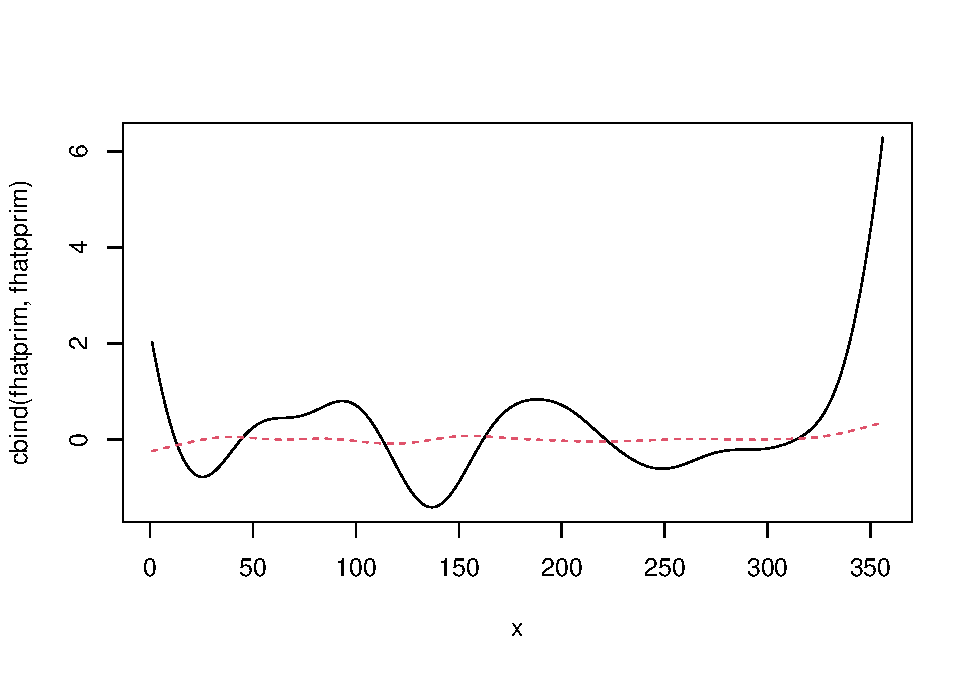
\includegraphics{Projet_CHESNAIS_GUIBERT_files/figure-latex/unnamed-chunk-27-1.pdf}

La dérivée première, en noir, correspondant à la vitesse de croissance,
n'est pas très lisse. Elle indique que par moment dans l'année, la
consommation d'énergie diminue ou augmente brusquement. Par exemple au
niveau du 20ème et 140ème jour, sa consommation d'énergie décroit
rapidement. A la fin de l'année, celle-ci explose.

Les dérivées obtenues sont régulières (on a pris une base d'ordre plus
élevé, égale à 6) et le lissage est contraint par la rugosité de la
dérivée seconde avec une pénalité sur la dérivée d'ordre 6.

\hypertarget{iii.b.-pour-lensemble-des-etats}{%
\subsection{III.B. Pour l'ensemble des
Etats}\label{iii.b.-pour-lensemble-des-etats}}

Nous allons généraliser notre démarche pour tous les Etats.

\uline{Lissage par moindre carrés pénalisés}

On fait l'ajustement pour différentes valeurs de lambda pour minimiser
le critère de pénalité.\\
On veut la fonction la plus proche des points et la moins oscillante
grâce à la pénalité.

\begin{Shaded}
\begin{Highlighting}[]
\CommentTok{\# Initialisation d\textquotesingle{}une grille de lambda}
\NormalTok{gcv }\OtherTok{=} \FunctionTok{rep}\NormalTok{(}\DecValTok{0}\NormalTok{,}\DecValTok{30}\NormalTok{) }

\ControlFlowTok{for}\NormalTok{ (i }\ControlFlowTok{in} \DecValTok{1}\SpecialCharTok{:}\DecValTok{30}\NormalTok{)\{}
\NormalTok{  lambda }\OtherTok{=} \FunctionTok{exp}\NormalTok{(i}\DecValTok{{-}10}\NormalTok{)}
\NormalTok{  fdpar }\OtherTok{=} \FunctionTok{fdPar}\NormalTok{(splbasis,}\AttributeTok{Lfdobj =} \DecValTok{4}\NormalTok{,}\AttributeTok{lambda=}\NormalTok{lambda)}
\NormalTok{  smoothdata }\OtherTok{=} \FunctionTok{smooth.basis}\NormalTok{(tps,}\FunctionTok{as.matrix}\NormalTok{(data\_long[,}\FunctionTok{c}\NormalTok{(}\SpecialCharTok{{-}}\DecValTok{1}\NormalTok{)]), }
                            \AttributeTok{fdParobj =}\NormalTok{ fdpar)}
\NormalTok{  gcv[i] }\OtherTok{=} \FunctionTok{mean}\NormalTok{(smoothdata}\SpecialCharTok{$}\NormalTok{gcv) }
\NormalTok{\}}
\FunctionTok{plot}\NormalTok{(gcv)}
\end{Highlighting}
\end{Shaded}

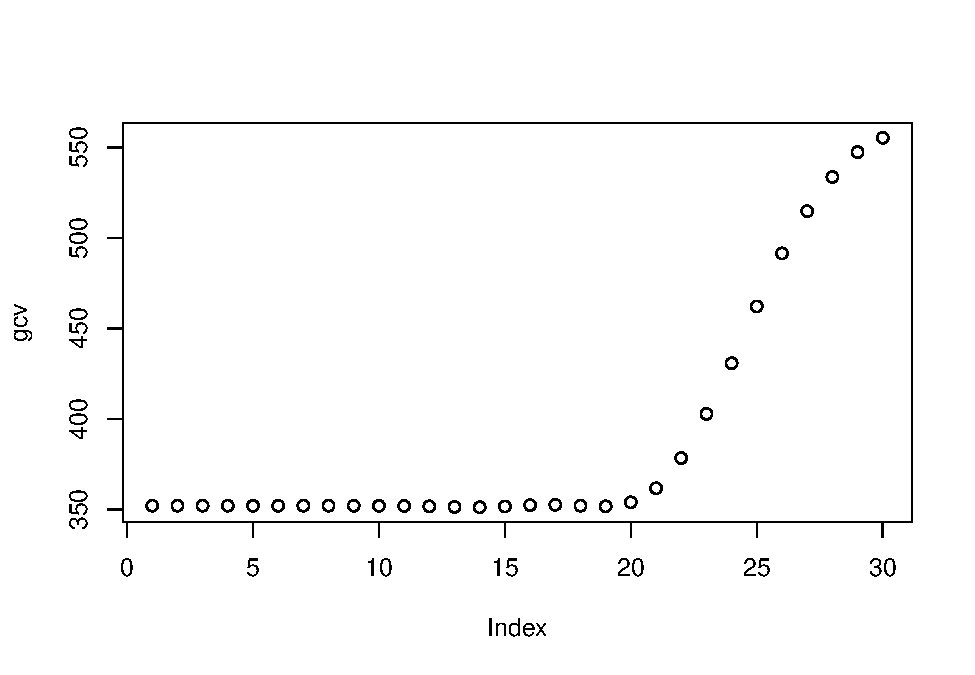
\includegraphics{Projet_CHESNAIS_GUIBERT_files/figure-latex/unnamed-chunk-28-1.pdf}

\begin{Shaded}
\begin{Highlighting}[]
\FunctionTok{which.min}\NormalTok{(gcv)}
\end{Highlighting}
\end{Shaded}

\begin{verbatim}
## [1] 14
\end{verbatim}

Nous avons observé que la valeur optimale de lambda est la 14ème valeur,
correspondant au minimum. Cette valeur nous permettra d'être proche des
données observées.\\
Nous avons choisi de paramétrer le nombre de coupures à 35 car les
signaux sont très irréguliers et nous souhaitons être proche, mais
raisonnablement, du signal d'origine. Ce choix est arbitraire car il
peut engendrer du sur-apprentissage si le nombre de coupures est trop
élevée par rapport au signal de départ.

Nous allons recalculer la pénalité et refaire le lissage avec la valeur
de lambda minimale :

\begin{Shaded}
\begin{Highlighting}[]
\NormalTok{lambda }\OtherTok{=} \FunctionTok{exp}\NormalTok{(}\FunctionTok{which.min}\NormalTok{(gcv)}\SpecialCharTok{{-}}\DecValTok{10}\NormalTok{)}
\NormalTok{fdpar }\OtherTok{=} \FunctionTok{fdPar}\NormalTok{(splbasis,}\AttributeTok{Lfdobj =} \DecValTok{4}\NormalTok{,}\AttributeTok{lambda=}\NormalTok{lambda) }\CommentTok{\# calcul pénalité}
\NormalTok{smoothdata }\OtherTok{=} \FunctionTok{smooth.basis}\NormalTok{(tps,}\FunctionTok{as.matrix}\NormalTok{(data\_long[,}\FunctionTok{c}\NormalTok{(}\SpecialCharTok{{-}}\DecValTok{1}\NormalTok{)]),}
                          \AttributeTok{fdParobj =}\NormalTok{ fdpar) }\CommentTok{\# lissage}
\end{Highlighting}
\end{Shaded}

Nous évaluons notre objet fonctionnel à chaque point de temps :

\begin{Shaded}
\begin{Highlighting}[]
\NormalTok{fhatsmooth }\OtherTok{\textless{}{-}} \FunctionTok{eval.fd}\NormalTok{(tps, smoothdata}\SpecialCharTok{$}\NormalTok{fd)}
\end{Highlighting}
\end{Shaded}

\uline{Représentation pour l'ensemble des Etats}

Nous représentons les observations et la fonction estimée reconstruite
ˆf.

\begin{Shaded}
\begin{Highlighting}[]
\FunctionTok{matplot}\NormalTok{(tps,data\_long[,}\FunctionTok{c}\NormalTok{(}\SpecialCharTok{{-}}\DecValTok{1}\NormalTok{)],}\AttributeTok{type=}\StringTok{"l"}\NormalTok{,}\AttributeTok{lty=}\DecValTok{1}\NormalTok{,}\AttributeTok{ylab=}\StringTok{""}\NormalTok{,}\AttributeTok{main=}\StringTok{"donnees brutes"}\NormalTok{)}
\end{Highlighting}
\end{Shaded}

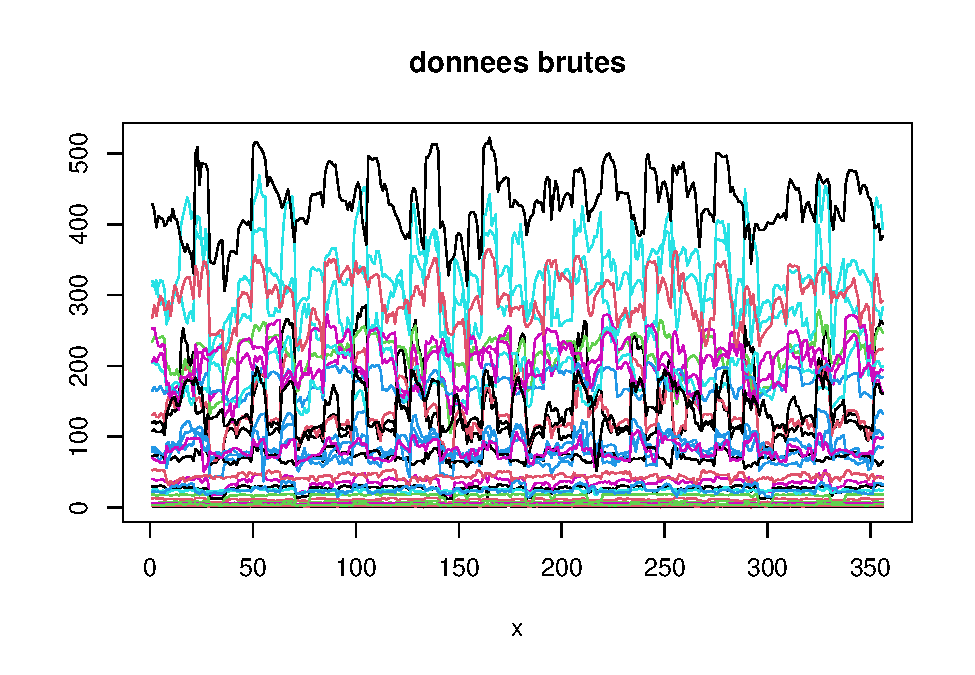
\includegraphics{Projet_CHESNAIS_GUIBERT_files/figure-latex/unnamed-chunk-31-1.pdf}

\begin{Shaded}
\begin{Highlighting}[]
\FunctionTok{matplot}\NormalTok{(tps,fhatsmooth,}\AttributeTok{type=}\StringTok{"l"}\NormalTok{,}\AttributeTok{lty=}\DecValTok{1}\NormalTok{,}\AttributeTok{ylab=}\StringTok{""}\NormalTok{,}\AttributeTok{main=}\StringTok{"donnees lissees"}\NormalTok{)}
\end{Highlighting}
\end{Shaded}

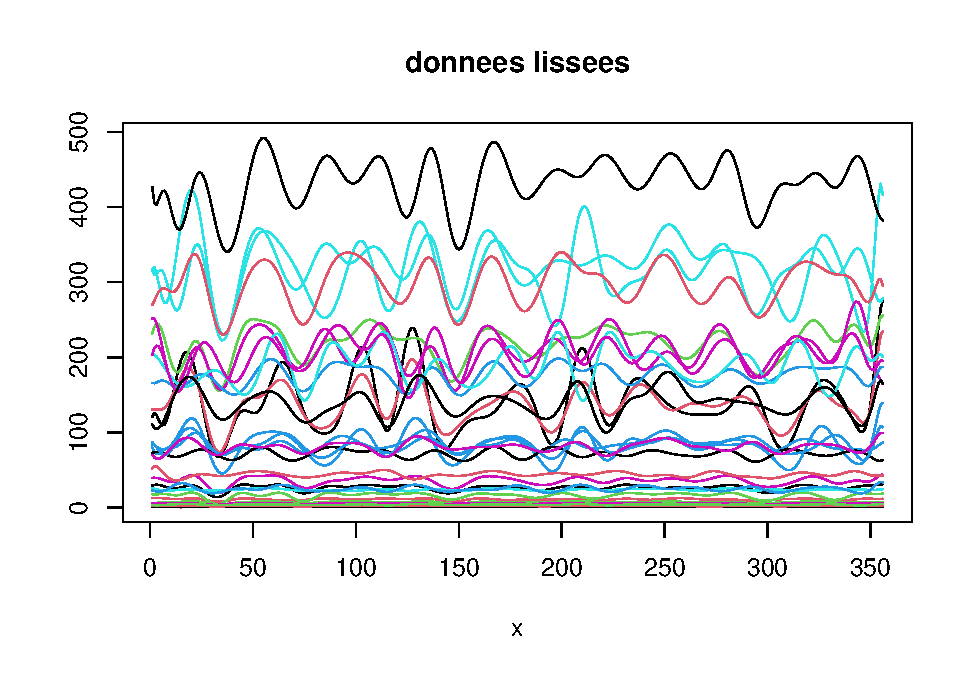
\includegraphics{Projet_CHESNAIS_GUIBERT_files/figure-latex/unnamed-chunk-31-2.pdf}

Nous obtenons des courbes lissées, moins irrégulières, qui explique bien
la tendance de la consommation d'énergie pour chacun des Etats.

Lors de la création de notre base de spline, nous avons choisi 35
coupures, ce qui biaise forcément notre analyse. Avec ces courbes
lissées, les analyses ne sont pas exhaustives pour éviter le
sur-apprentissage. Avec cette représentation, nous pouvons supposer
qu'il y a plus de variabilité en hiver (première partie de l'année)
qu'en été. Il faudrait un expert pour nous aiguiller sur ce sujet.

Nous représentons maintenant la dérivée première et seconde pour étudier
les vitesses de croissance et les accélérations de croissance.

\begin{Shaded}
\begin{Highlighting}[]
\NormalTok{fhatprim }\OtherTok{=} \FunctionTok{eval.fd}\NormalTok{(tps,smoothdata}\SpecialCharTok{$}\NormalTok{fd,}\AttributeTok{Lfdobj=}\DecValTok{1}\NormalTok{) }\CommentTok{\# dérivé première}
\NormalTok{fhatpprim }\OtherTok{=} \FunctionTok{eval.fd}\NormalTok{(tps,smoothdata}\SpecialCharTok{$}\NormalTok{fd,}\AttributeTok{Lfdobj=}\DecValTok{2}\NormalTok{) }\CommentTok{\# dérivé seconde}
\FunctionTok{matplot}\NormalTok{(tps,}
\NormalTok{        fhatprim,}
        \AttributeTok{type=}\StringTok{"l"}\NormalTok{,}
        \AttributeTok{main =} \StringTok{"Dérivée première"}\NormalTok{)}
\end{Highlighting}
\end{Shaded}

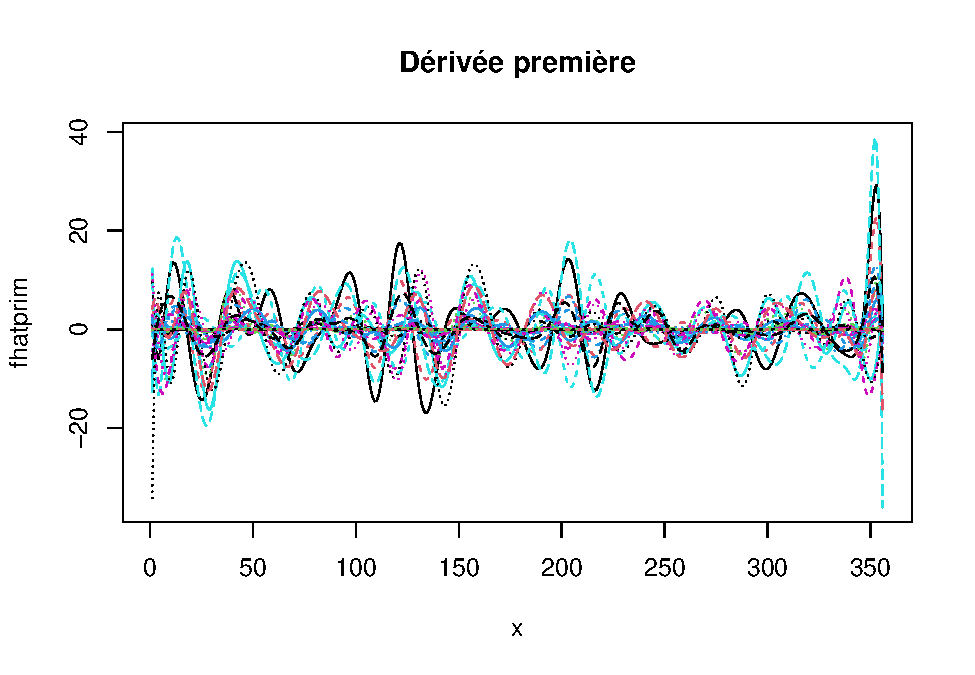
\includegraphics{Projet_CHESNAIS_GUIBERT_files/figure-latex/unnamed-chunk-32-1.pdf}

\begin{Shaded}
\begin{Highlighting}[]
\FunctionTok{matplot}\NormalTok{(tps, fhatpprim, }\AttributeTok{type =} \StringTok{"l"}\NormalTok{,}
        \AttributeTok{main =} \StringTok{"Dérivée seconde"}\NormalTok{)}
\end{Highlighting}
\end{Shaded}

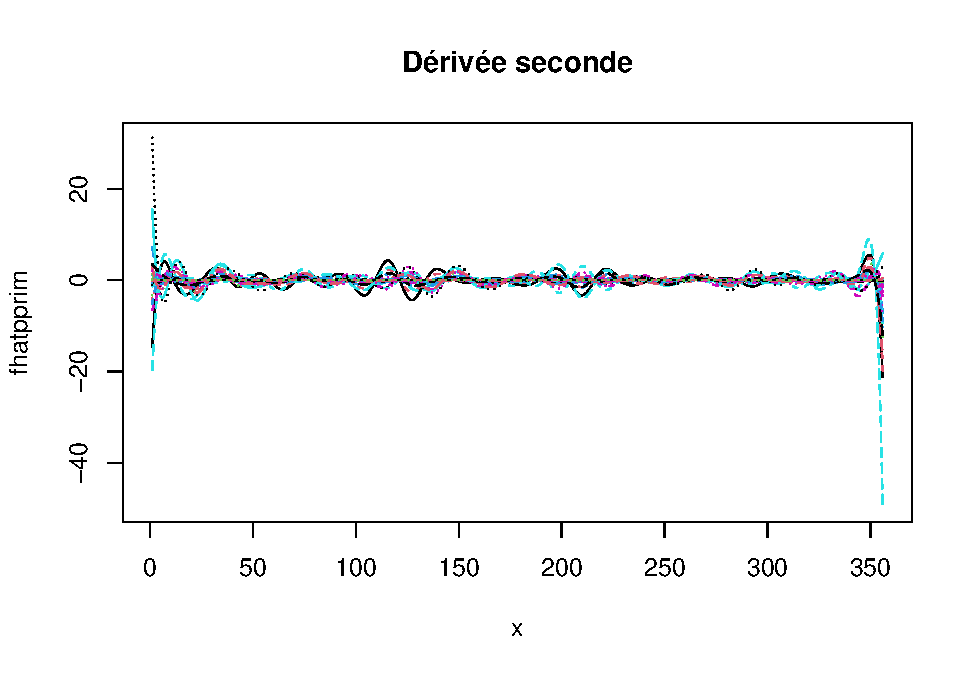
\includegraphics{Projet_CHESNAIS_GUIBERT_files/figure-latex/unnamed-chunk-32-2.pdf}
Les dérivés premières montrent des fluctuations, ce qui implique des
différences de vitesse de consommation dans les différents Etats.

\hypertarget{iv.-statistiques-exploratoires}{%
\section{IV. Statistiques
exploratoires}\label{iv.-statistiques-exploratoires}}

Nous allons réaliser quelques statistiques exploratoires pour pouvoir
appréhender au mieux les données et détecter les pays avec un
comportement atypique.

\hypertarget{iv.a.-moyenne-fonctionnelle}{%
\subsection{IV.A. Moyenne
fonctionnelle}\label{iv.a.-moyenne-fonctionnelle}}

Afin de visualiser les tendances, nous allons représenter la moyenne de
notre objet fonctionnel.

\begin{Shaded}
\begin{Highlighting}[]
\NormalTok{mean\_smooth\_data }\OtherTok{=} \FunctionTok{mean.fd}\NormalTok{(smoothdata}\SpecialCharTok{$}\NormalTok{fd)}
\CommentTok{\# mean\_smooth\_data}
\end{Highlighting}
\end{Shaded}

\begin{Shaded}
\begin{Highlighting}[]
\FunctionTok{matplot}\NormalTok{(fhatsmooth,}\AttributeTok{col=}\StringTok{"gray"}\NormalTok{,}\AttributeTok{type=}\StringTok{"l"}\NormalTok{,}
        \AttributeTok{xlab=}\StringTok{"jours"}\NormalTok{,}
        \AttributeTok{ylab=}\StringTok{"Consommation d\textquotesingle{}énergie"}\NormalTok{, }
        \AttributeTok{main =} \StringTok{"Consommation d\textquotesingle{}énergie des Etats d\textquotesingle{}Inde, }\SpecialCharTok{\textbackslash{}n}\StringTok{ avec tracé de la moyenne"}
\NormalTok{        )}
\FunctionTok{lines}\NormalTok{(mean\_smooth\_data,}\AttributeTok{lwd=}\DecValTok{2}\NormalTok{) }\CommentTok{\# moyenne}
\end{Highlighting}
\end{Shaded}

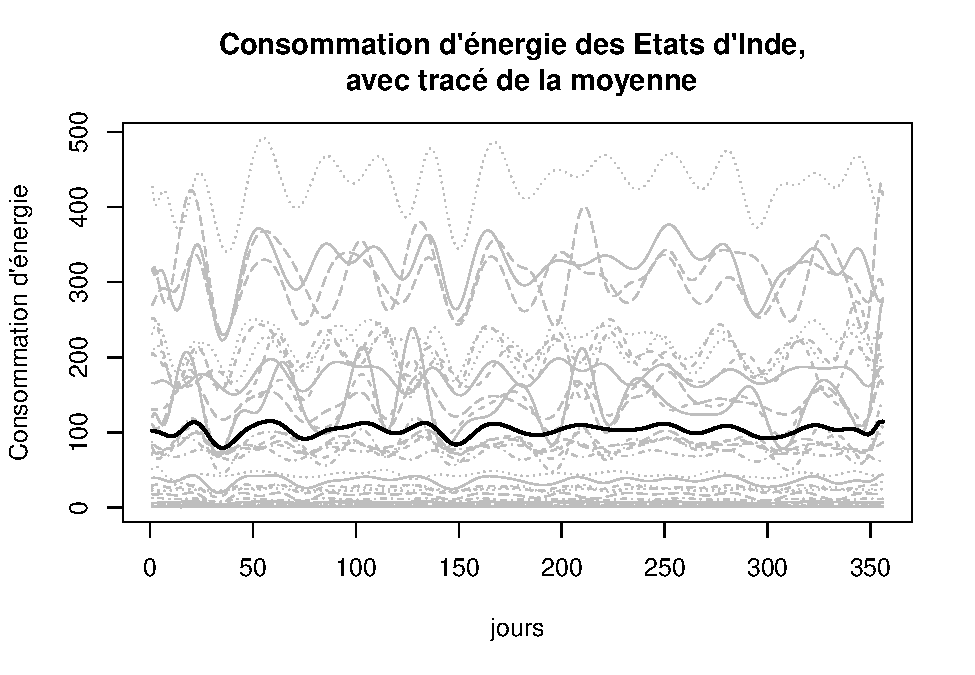
\includegraphics{Projet_CHESNAIS_GUIBERT_files/figure-latex/unnamed-chunk-34-1.pdf}

Grâce à ce graphique, nous pouvons observer la courbe moyenne de la
consommation d'énergie dans les différents Etats d'Inde. Les valeurs de
consommations sont situées aux alentours de 100 Méga Units.\\
Cette courbe est influencée par les valeurs extrêmes car nous pouvons
observer un grand nombre de courbes avec des valeurs plus faibles de
consommation.

\hypertarget{iv.b.-ecart-type-fonctionnel}{%
\subsection{IV.B. Ecart-type
fonctionnel}\label{iv.b.-ecart-type-fonctionnel}}

La représentation de l'écart-type fonctionnel permet de caractériser la
variabilité de nos signaux sur la période étudiée.\\
Nous allons pouvoir identifier s'il existe des périodes de stabilité ou
d'instabilité entre le début et la fin de l'année 2019.\\
Aussi, nous allons pouvoir comparer les différents Etats pour analyser
d'éventuels similarités ou différences.

\begin{Shaded}
\begin{Highlighting}[]
\NormalTok{sd\_smooth\_data}\OtherTok{=} \FunctionTok{sd.fd}\NormalTok{(smoothdata}\SpecialCharTok{$}\NormalTok{fd)}
\end{Highlighting}
\end{Shaded}

\begin{Shaded}
\begin{Highlighting}[]
\FunctionTok{matplot}\NormalTok{(fhatsmooth,}
        \AttributeTok{col=}\StringTok{"gray"}\NormalTok{,}\AttributeTok{type=}\StringTok{"l"}\NormalTok{,}
        \AttributeTok{xlab=}\StringTok{"jours"}\NormalTok{,}
        \AttributeTok{ylab=}\StringTok{"Consommation d\textquotesingle{}énergie"}\NormalTok{,}
        \AttributeTok{ylim =} \FunctionTok{c}\NormalTok{(}\SpecialCharTok{{-}}\DecValTok{200}\NormalTok{,}\DecValTok{500}\NormalTok{))}
\NormalTok{fnmoy }\OtherTok{=} \FunctionTok{eval.fd}\NormalTok{(y,mean\_smooth\_data)}
\NormalTok{fnsd  }\OtherTok{=} \FunctionTok{eval.fd}\NormalTok{(y,sd\_smooth\_data)}
\FunctionTok{lines}\NormalTok{(fnmoy,}\AttributeTok{lwd=}\DecValTok{2}\NormalTok{)}
\FunctionTok{lines}\NormalTok{(fnmoy}\SpecialCharTok{+}\DecValTok{2}\SpecialCharTok{*}\NormalTok{fnsd,}\AttributeTok{lwd=}\DecValTok{2}\NormalTok{,}\AttributeTok{col=}\DecValTok{4}\NormalTok{,}\AttributeTok{lty=}\DecValTok{2}\NormalTok{)}
\FunctionTok{lines}\NormalTok{(fnmoy}\DecValTok{{-}2}\SpecialCharTok{*}\NormalTok{fnsd,}\AttributeTok{lwd=}\DecValTok{2}\NormalTok{,}\AttributeTok{col=}\DecValTok{4}\NormalTok{,}\AttributeTok{lty=}\DecValTok{2}\NormalTok{)}
\end{Highlighting}
\end{Shaded}

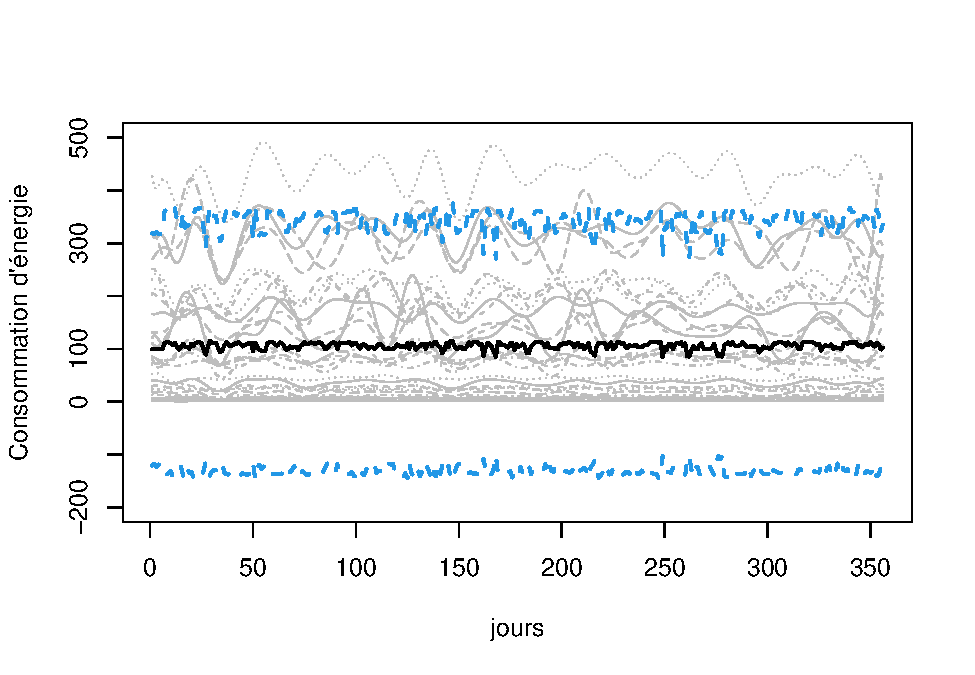
\includegraphics{Projet_CHESNAIS_GUIBERT_files/figure-latex/unnamed-chunk-36-1.pdf}

Ce graphique nous permet de visualiser les consommations d'énergie
(données lissées) des différents Etats en Inde. La courbe moyenne, en
noir, nous permet d'avoir une idée de la tendance centrale. La plage de
variabilité est définie par les pointillés en bleus, correspondant à la
moyenne plus (ou moins) 2 fois l'écart-type.\\
La majorité des pays présentent donc des données lissées proches de la
moyenne. Nous pouvons identifier quelques Etats atypiques.

\hypertarget{iv.c.-surface-de-covariance-et-corruxe9lation}{%
\subsection{IV.C. Surface de covariance et
corrélation}\label{iv.c.-surface-de-covariance-et-corruxe9lation}}

Afin d'explorer les relations et les dépendances entre nos différents
Etats.

\hypertarget{iv.c.1.-covariance}{%
\subsubsection{IV.C.1. Covariance}\label{iv.c.1.-covariance}}

Dans un premier temps, nous allons mesurer comment les consommations des
Etats évoluent conjointement en fonction du temps.

\begin{Shaded}
\begin{Highlighting}[]
\NormalTok{cov }\OtherTok{=} \FunctionTok{var.fd}\NormalTok{(smoothdata}\SpecialCharTok{$}\NormalTok{fd)}
\NormalTok{surfcov }\OtherTok{=} \FunctionTok{eval.bifd}\NormalTok{(}\FunctionTok{seq}\NormalTok{(}\DecValTok{1}\NormalTok{,}\DecValTok{356}\NormalTok{,}\AttributeTok{length=}\DecValTok{35}\NormalTok{),}\FunctionTok{seq}\NormalTok{(}\DecValTok{1}\NormalTok{,}\DecValTok{356}\NormalTok{,}\AttributeTok{length=}\DecValTok{35}\NormalTok{),cov)}
\end{Highlighting}
\end{Shaded}

Pour le tracé d'une surface, il est préférable de choisir un nombre
modéré de points dans la grille d'évaluation (la représentation est
rapidement illisible dans le cas contraire). Ici, nous choisissons
arbitrairement 30 points répartis entre 1 et 356.

\begin{Shaded}
\begin{Highlighting}[]
\FunctionTok{persp}\NormalTok{(surfcov,}\AttributeTok{col=}\StringTok{"gray"}\NormalTok{,}\AttributeTok{theta=}\DecValTok{30}\NormalTok{,}\AttributeTok{xlab=}\StringTok{"jours"}\NormalTok{,}\AttributeTok{ylab=}\StringTok{"jours"}\NormalTok{,}\AttributeTok{zlab=}\StringTok{"covariance"}\NormalTok{)}
\end{Highlighting}
\end{Shaded}

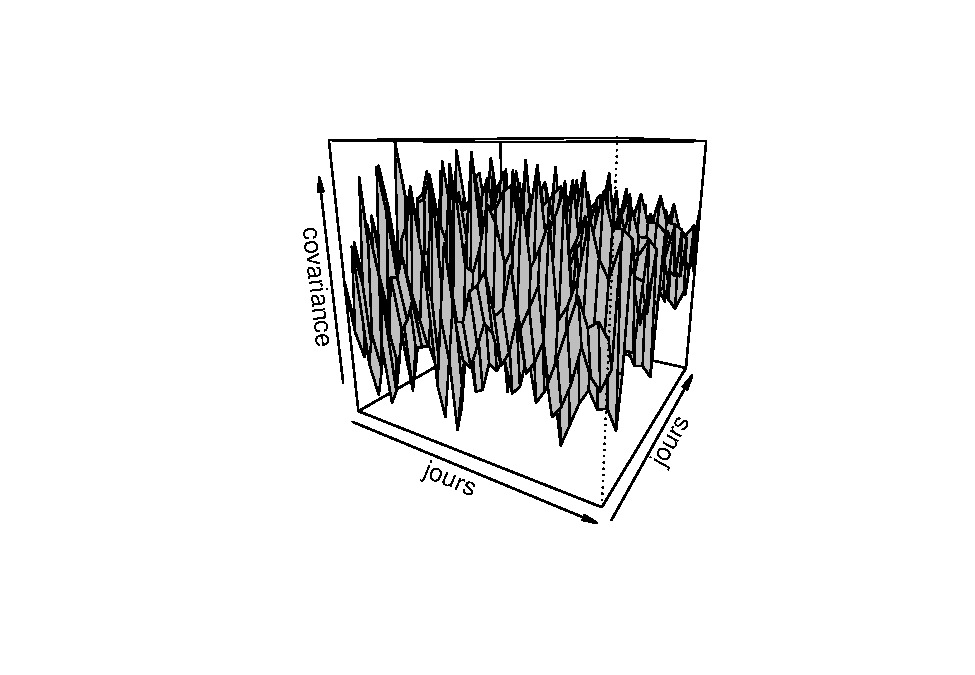
\includegraphics{Projet_CHESNAIS_GUIBERT_files/figure-latex/unnamed-chunk-38-1.pdf}

L'analyse de cette représentation est assez compliquée car elle permet
de visualiser la covariance entre les différentes consommations des
Etats selon les jours, mais aucune tendance claire ne se dégage.

\begin{Shaded}
\begin{Highlighting}[]
\FunctionTok{contour}\NormalTok{(surfcov)}
\end{Highlighting}
\end{Shaded}

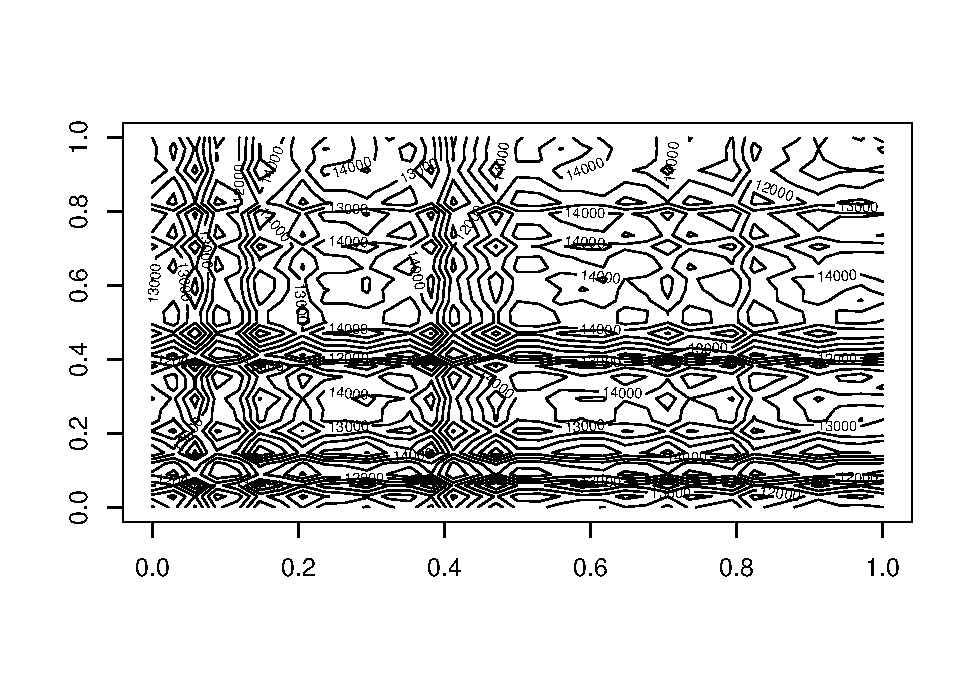
\includegraphics{Projet_CHESNAIS_GUIBERT_files/figure-latex/unnamed-chunk-39-1.pdf}

De même, cette représentation devraient pouvoir nous aider pour
identifier la covariance entre les consommations d'énergie des Etats
selon les jours mais il est presque illisible.

\hypertarget{iv.c.2.-repruxe9sentation-graphique-en-couleur}{%
\subsubsection{IV.C.2. Représentation graphique en
couleur}\label{iv.c.2.-repruxe9sentation-graphique-en-couleur}}

\begin{Shaded}
\begin{Highlighting}[]
\FunctionTok{filled.contour}\NormalTok{(surfcov)}
\end{Highlighting}
\end{Shaded}

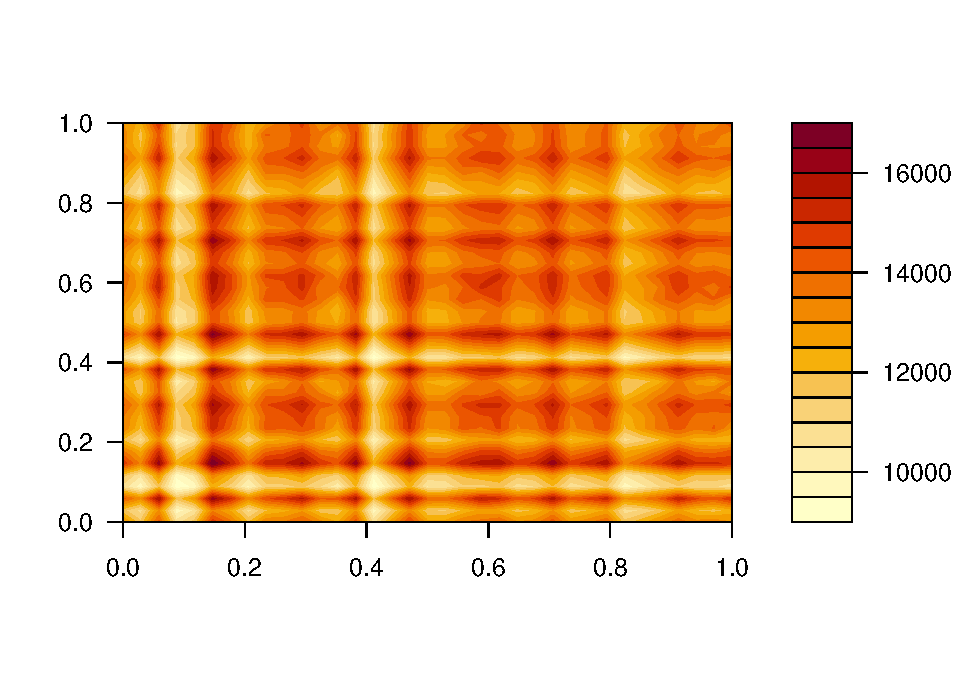
\includegraphics{Projet_CHESNAIS_GUIBERT_files/figure-latex/unnamed-chunk-40-1.pdf}

En général, on peut voir que la covariance est ``moyenne'' entre le
début et la fin de l'année pour chaque Etat. Nous pouvons observer des
moments où la covariance est moins importante, autour du mois d'Avril
(0.4) et de Septembre (0.8).

\hypertarget{iv.c.3.-corruxe9lation}{%
\subsubsection{IV.C.3. Corrélation}\label{iv.c.3.-corruxe9lation}}

L'analyse de la corrélation nous permet de détecter si nous avons des
effets d'un jour à l'autre sur la consommation d'Energie dans les divers
Etats d'Inde.

Nous construisons d'abord la matrice de corrélation :

\begin{Shaded}
\begin{Highlighting}[]
\NormalTok{cor }\OtherTok{=} \FunctionTok{cor.fd}\NormalTok{(}\FunctionTok{seq}\NormalTok{(}\DecValTok{1}\NormalTok{,}\DecValTok{356}\NormalTok{,}\AttributeTok{length=}\DecValTok{35}\NormalTok{),smoothdata}\SpecialCharTok{$}\NormalTok{fd)}
\CommentTok{\# cor}
\end{Highlighting}
\end{Shaded}

Cette manipulation nous permet de récupérer la matrice de corrélation
empirique évaluée (sur les données lissées) en chaque point de temps
(jour).

Nous allons représenter graphiquement la matrice de corrélation :

\begin{Shaded}
\begin{Highlighting}[]
\FunctionTok{persp}\NormalTok{(cor,}\AttributeTok{col=}\StringTok{"gray"}\NormalTok{,}\AttributeTok{theta=}\DecValTok{90}\NormalTok{,}
      \AttributeTok{phi=}\DecValTok{40}\NormalTok{,}\AttributeTok{xlab=}\StringTok{"jours"}\NormalTok{,}
      \AttributeTok{ylab=}\StringTok{"jours"}\NormalTok{,}\AttributeTok{zlab=}\StringTok{"corrélation"}\NormalTok{)}
\end{Highlighting}
\end{Shaded}

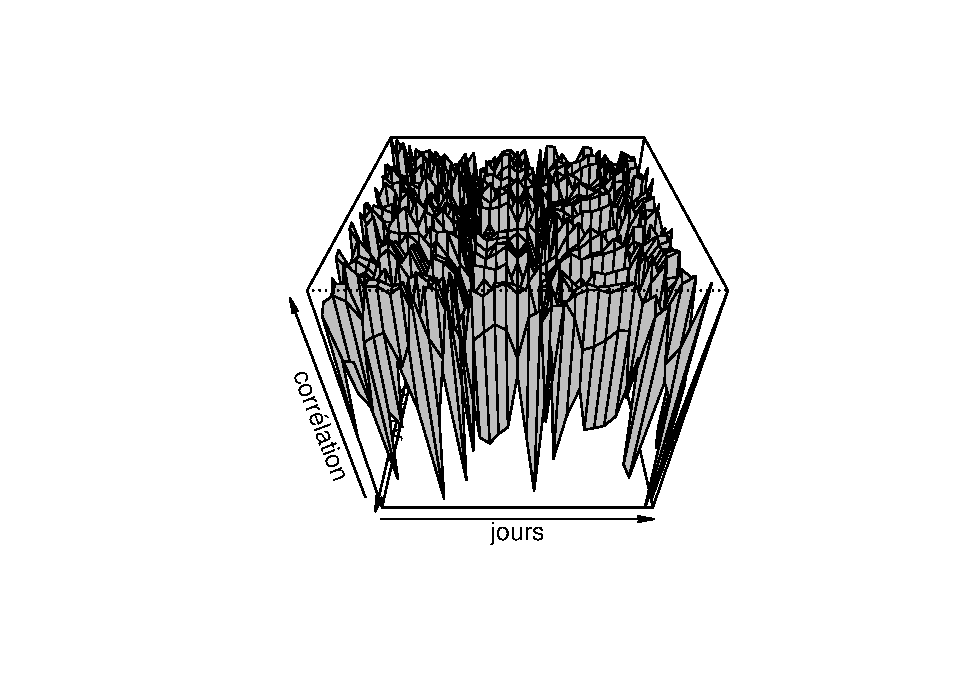
\includegraphics{Projet_CHESNAIS_GUIBERT_files/figure-latex/unnamed-chunk-42-1.pdf}

La corrélation est difficilement interprétable sur le graphe, nous
allons essayer une autre méthode.

\hypertarget{iv.c.4.-repruxe9sentation-graphique-en-couleur}{%
\subsubsection{IV.C.4. Représentation graphique en
couleur}\label{iv.c.4.-repruxe9sentation-graphique-en-couleur}}

\begin{Shaded}
\begin{Highlighting}[]
\FunctionTok{filled.contour}\NormalTok{(cor)}
\end{Highlighting}
\end{Shaded}

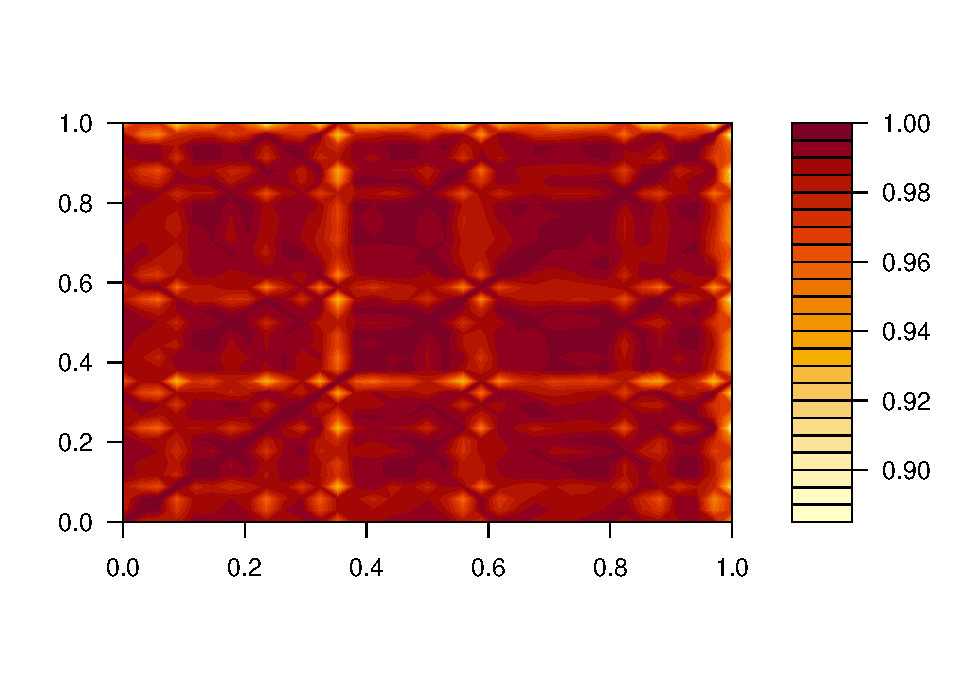
\includegraphics{Projet_CHESNAIS_GUIBERT_files/figure-latex/unnamed-chunk-43-1.pdf}

Nous pouvons observer une corrélation égale à 1 sur la diagonale car la
consommation d'un jour est forcément corrélée avec elle-même.\\
De plus, nous pouvons voir que les corrélations sont globalement fortes
d'un jour à l'autre, ce qui signifie que la consommation de la veille
influence celle du lendemain.

\hypertarget{iv.d.-acp-fonctionnelle}{%
\subsection{IV.D. ACP fonctionnelle}\label{iv.d.-acp-fonctionnelle}}

\begin{Shaded}
\begin{Highlighting}[]
\NormalTok{ACPF }\OtherTok{=} \FunctionTok{pca.fd}\NormalTok{(smoothdata}\SpecialCharTok{$}\NormalTok{fd,}\AttributeTok{nharm=}\DecValTok{4}\NormalTok{,}\AttributeTok{centerfns =} \ConstantTok{TRUE}\NormalTok{)}
\NormalTok{ACPF}\SpecialCharTok{$}\NormalTok{varprop}
\end{Highlighting}
\end{Shaded}

\begin{verbatim}
## [1] 0.987179812 0.008252207 0.001454582 0.001198720
\end{verbatim}

\begin{Shaded}
\begin{Highlighting}[]
\FunctionTok{cumsum}\NormalTok{(ACPF}\SpecialCharTok{$}\NormalTok{varprop)}
\end{Highlighting}
\end{Shaded}

\begin{verbatim}
## [1] 0.9871798 0.9954320 0.9968866 0.9980853
\end{verbatim}

La première composante explique environ 99\% de la variabilité.

\hypertarget{iv.d.1.-repruxe9sentations-des-composantes-principales}{%
\subsubsection{IV.D.1. Représentations des composantes
principales}\label{iv.d.1.-repruxe9sentations-des-composantes-principales}}

Nous représentons en premier lieu les composantes principales obtenues

\begin{Shaded}
\begin{Highlighting}[]
\FunctionTok{plot}\NormalTok{(ACPF}\SpecialCharTok{$}\NormalTok{harmonics)}
\end{Highlighting}
\end{Shaded}

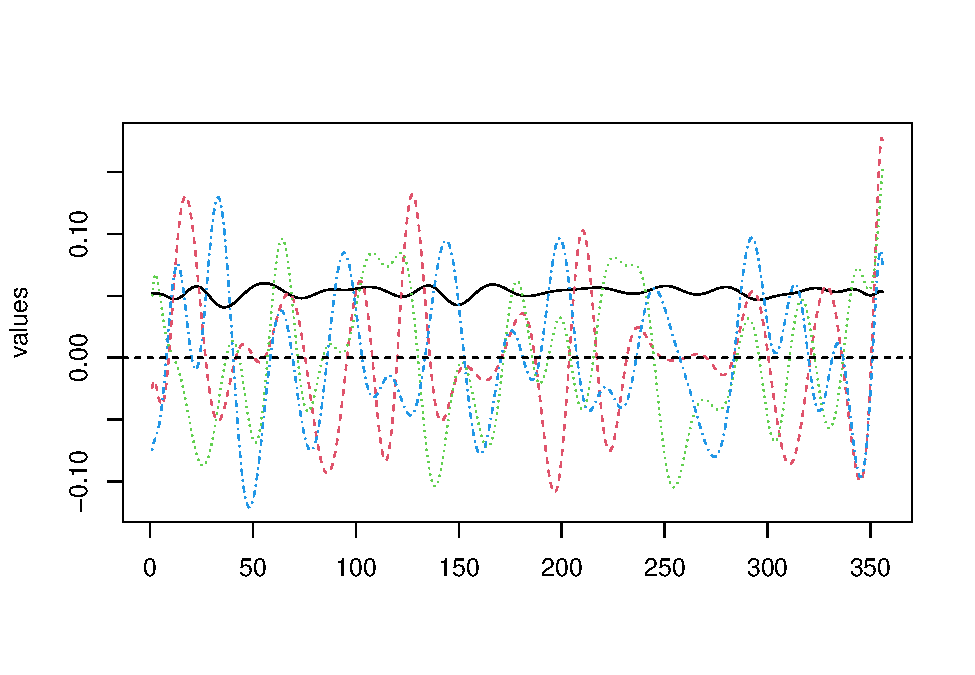
\includegraphics{Projet_CHESNAIS_GUIBERT_files/figure-latex/unnamed-chunk-45-1.pdf}

\begin{verbatim}
## [1] "done"
\end{verbatim}

La première composante (en noir) est tout le temps positive.
Globalement, elle a quelques variations, environ au 30ème, 140ème et
280ème jour de l'année. Elle a donc tendance à être plus élevé en hiver.

Pour une interprétation plus aisée, on représente la moyenne augmentée
ou diminuée des premières fonctions propres.

On peut utilisée la fonction \texttt{plot.pca.fd} pour cette
représentation.

\begin{Shaded}
\begin{Highlighting}[]
\FunctionTok{plot.pca.fd}\NormalTok{(ACPF)}
\end{Highlighting}
\end{Shaded}

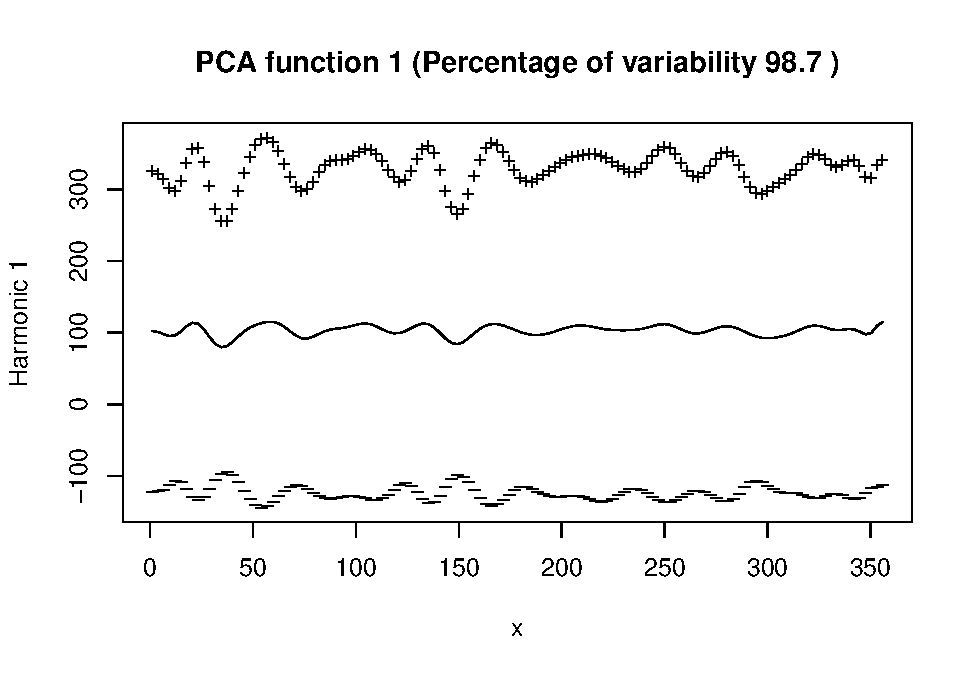
\includegraphics{Projet_CHESNAIS_GUIBERT_files/figure-latex/unnamed-chunk-46-1.pdf}
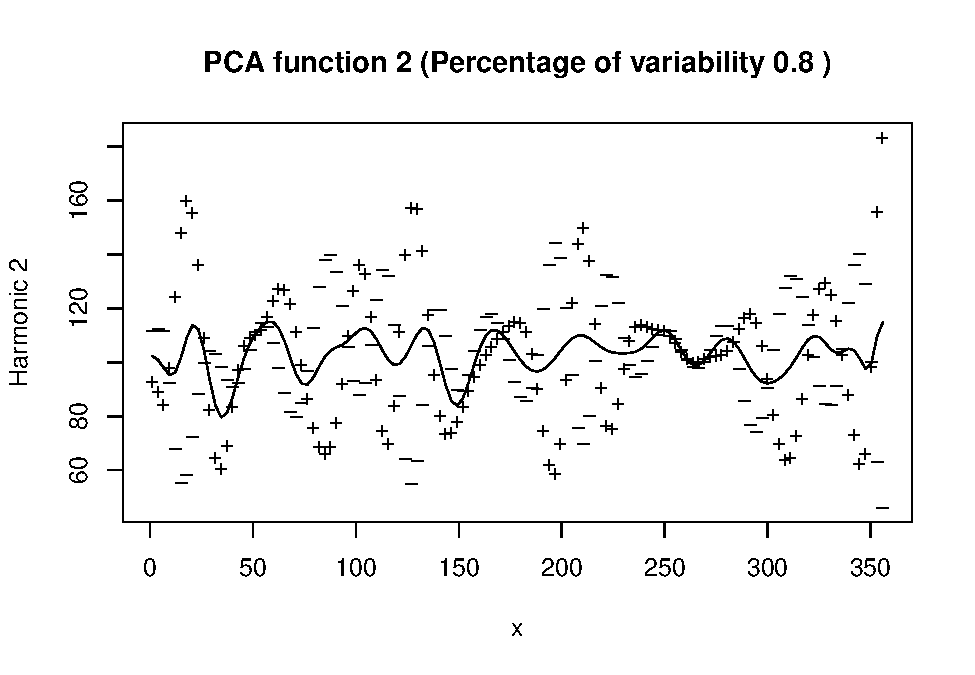
\includegraphics{Projet_CHESNAIS_GUIBERT_files/figure-latex/unnamed-chunk-46-2.pdf}
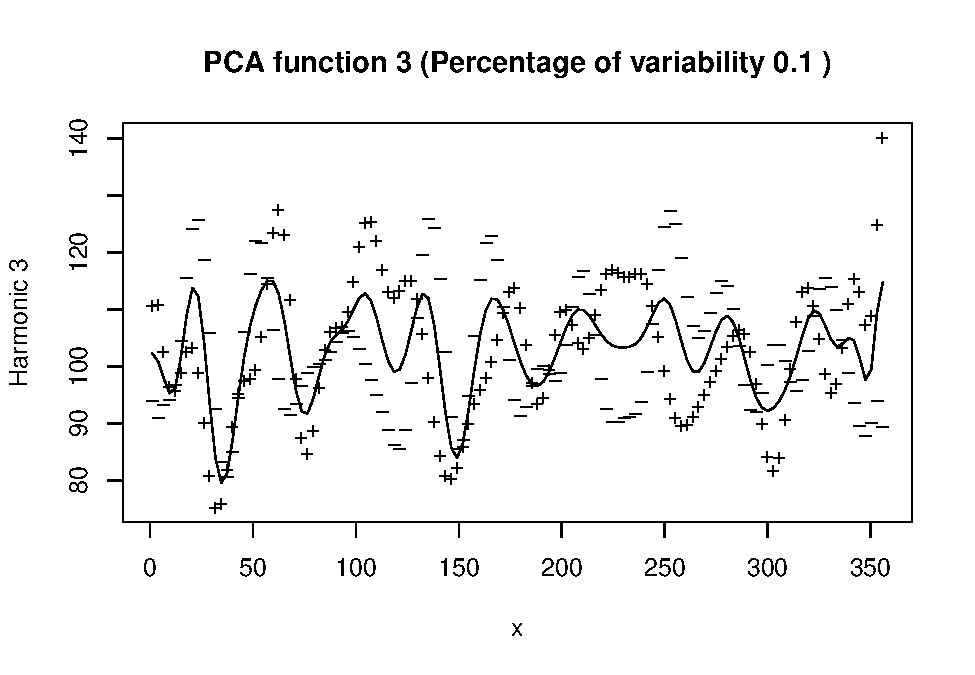
\includegraphics{Projet_CHESNAIS_GUIBERT_files/figure-latex/unnamed-chunk-46-3.pdf}
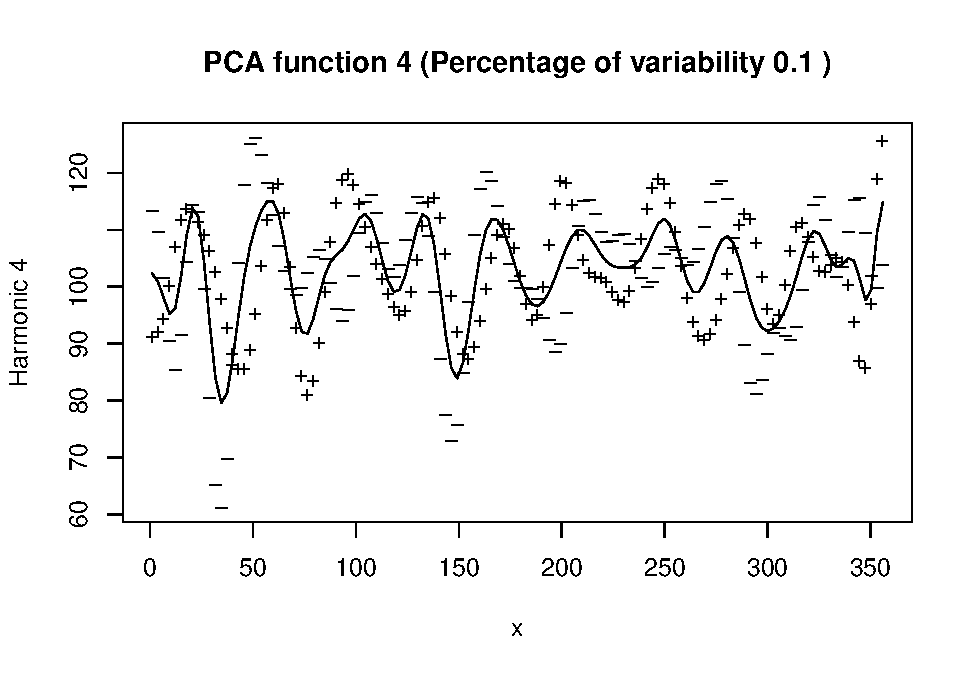
\includegraphics{Projet_CHESNAIS_GUIBERT_files/figure-latex/unnamed-chunk-46-4.pdf}

Pour la première fonction propre:

\begin{itemize}
\item
  La courbe en noir représente la moyenne
\item
  La courbe avec des ``-'' représente la moyenne - alpha * la première
  composantes principales
\item
  La courbe avec des ``+'' représente la moyenne + alpha * la première
  composantes principales
\end{itemize}

Comme évoqué précédemment, nous pouvons supposer qu'il y a plus de
variabilité en hiver qu'en été.

\hypertarget{iv.d.2.-repruxe9sentation-des-individus}{%
\subsubsection{IV.D.2. Représentation des
individus}\label{iv.d.2.-repruxe9sentation-des-individus}}

\uline{Représentation des individus dans le premier plan factoriel}

Les scores des individus sont stockés dans la matrice \texttt{scores} de
\texttt{ACPF}. Nous allons les représenter sur le premier plan
factoriel.

\begin{Shaded}
\begin{Highlighting}[]
\FunctionTok{head}\NormalTok{(ACPF}\SpecialCharTok{$}\NormalTok{scores)}
\end{Highlighting}
\end{Shaded}

\begin{verbatim}
##            [,1]      [,2]       [,3]        [,4]
## [1,]   694.4987 574.65950  211.59702   -1.507536
## [2,]   652.9611 341.00037  133.02690  -38.626858
## [3,]  2182.0635 -35.48669  162.31803 -138.399753
## [4,]  -380.1501 242.24678  -11.92453  -35.326778
## [5,]  4004.6725 595.76303 -146.66314   12.226365
## [6,] -1259.7014  -5.22891    1.44213  -34.825769
\end{verbatim}

\begin{Shaded}
\begin{Highlighting}[]
\FunctionTok{plot}\NormalTok{(ACPF}\SpecialCharTok{$}\NormalTok{scores[,}\DecValTok{1}\NormalTok{],}
\NormalTok{     ACPF}\SpecialCharTok{$}\NormalTok{scores[,}\DecValTok{2}\NormalTok{],}
     \AttributeTok{pch=}\DecValTok{20}\NormalTok{,}
     \AttributeTok{xlab=}\StringTok{"FPC 1"}\NormalTok{,}
     \AttributeTok{ylab=}\StringTok{"FPC 2"}\NormalTok{,}
     \AttributeTok{type=}\StringTok{"n"}\NormalTok{)}
\NormalTok{nomsvilles }\OtherTok{=} \FunctionTok{colnames}\NormalTok{(data\_long[,}\FunctionTok{c}\NormalTok{(}\SpecialCharTok{{-}}\DecValTok{1}\NormalTok{)])}
\NormalTok{regions }\OtherTok{=} \FunctionTok{as.factor}\NormalTok{(data}\SpecialCharTok{$}\NormalTok{Regions)}
\FunctionTok{text}\NormalTok{(ACPF}\SpecialCharTok{$}\NormalTok{scores[,}\DecValTok{1}\NormalTok{],}
\NormalTok{     ACPF}\SpecialCharTok{$}\NormalTok{scores[,}\DecValTok{2}\NormalTok{],}
     \AttributeTok{labels=}\NormalTok{nomsvilles,}\AttributeTok{cex=}\FloatTok{0.7}\NormalTok{,}\AttributeTok{col=}\FunctionTok{as.numeric}\NormalTok{(regions))}
\FunctionTok{legend}\NormalTok{(}\StringTok{"topleft"}\NormalTok{,}\AttributeTok{legend =} \FunctionTok{levels}\NormalTok{(regions),}\AttributeTok{col=}\DecValTok{1}\SpecialCharTok{:}\DecValTok{4}\NormalTok{,}\AttributeTok{lty=}\DecValTok{1}\NormalTok{)}
\end{Highlighting}
\end{Shaded}

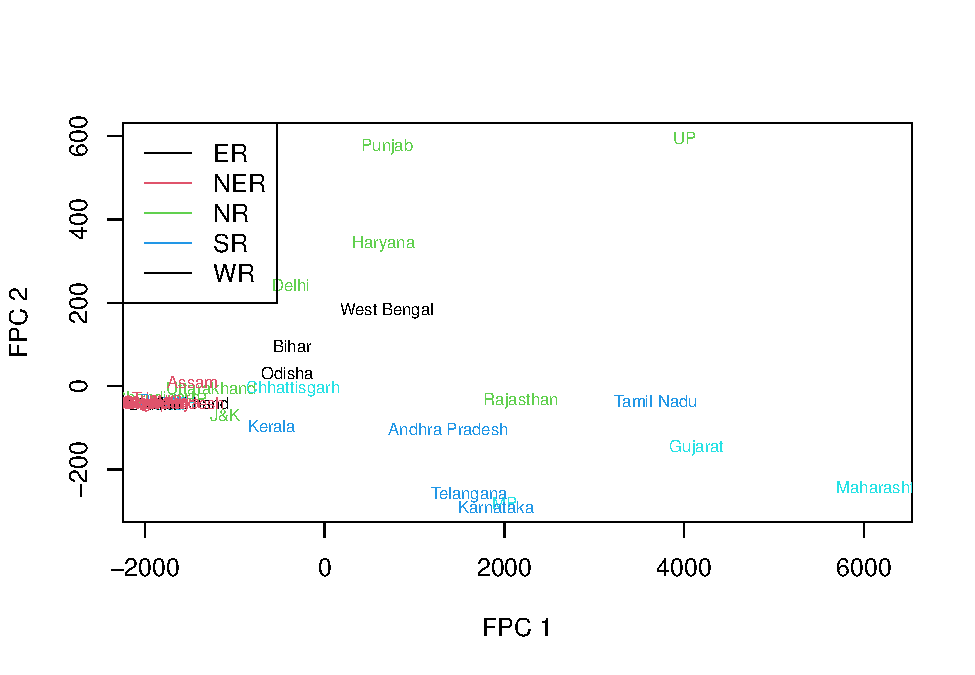
\includegraphics{Projet_CHESNAIS_GUIBERT_files/figure-latex/unnamed-chunk-47-1.pdf}

Aucune région ne semble se distinguer concernant les consommations
d'énergie des Etats. Cependant, nous observons quelques exceptions comme
la région NR (Nord) où quelques Etats présentent des valeurs assez
élevées sur le second axe factoriel contrairement à la région SR (Sud)
où les valeurs sont plutôt faibles.

Pour la première compostante principale (abscisse), les Etats concentrés
à droite du graphique présentent des valeurs de consommations d'énergie
élevées. Par exemple, Maharashtra et l'Etat du Gujarat sont des grands
consommateurs d'énergies. Pour les petites valeurs, les Etats présentent
des consommations plus faibles. Cette observation est en adéquation avec
les premières représentations graphiques que nous avons réalisées au
début de ce rapport.

Pour la deuxième composante principale (ordonnée), pour les Etats situés
en haut du graphique, cela indique que leur consommation d'énergie est
très variable selon les périodes de l'année. L'Etat du Punjab et Uttar
Pradesh (UP) présentent beaucoup d'écarts de valeurs. ~ Pour les petites
valeurs, cela signifie que les Etats ont des consommations d'énergie
plus stables entre le début et la fin de la période étudiée.

\hypertarget{v.-conclusion}{%
\section{V. Conclusion}\label{v.-conclusion}}

Pour rappel, nous avons analysé la consommation d'énergie dans les 33
Etats d'Inde. Pour cela, nous avons réalisé un lissage pénalisé avec des
bases de splines. Cette méthode est efficace pour modéliser et
représenter les tendances complexes des données. En utilisant ces
splines, nous avons pu capturer les variations locales tout en
maintenant une certaine régularite. Cela permet une visualisation plus
claire des motifs sous-jacents. De plus, cela permet de révéler des
tendances significatives et réduire le bruit, offrant ainsi une
meilleure compréhension de la dynamique de la consommation d'énergie
dans ces différents Etats d'Inde.

Nous avons pu mettre en évidence des disparités entre les Etats mais
aussi entre les régions de l'Inde. L'avis d'experts sur ce sujet nous
permettraient de compléter notre analyse et optimiser cette consommation
d'énergie pour limiter son impact sur l'environnement.

\hypertarget{vi.-sources}{%
\section{VI. Sources}\label{vi.-sources}}

\begin{itemize}
\tightlist
\item
  base de données :
  \url{https://www.kaggle.com/datasets/twinkle0705/state-wise-power-consumption-in-india?fbclid=IwAR3tNVrXpTrRlO_HVOoa53bcaTR8aR7QU_Nlbe4AhhmfzdK9ERa5Xxid1yk}
\end{itemize}

\end{document}
